\documentclass[12pt,a4paper,french]{report}
\usepackage{babel}
\usepackage{color}
\usepackage{hyperref}
\usepackage{graphicx}

\renewcommand \( { \left( }
\renewcommand \) { \right) }
\renewcommand \[ { \left[ }
\renewcommand \] { \right] }
\newcommand   \matlab {{\scriptsize {\it MATLAB$^{\copyright}$}} }
\newcommand   \matlabv {{\scriptsize {\it MATLAB$^{\copyright}$}}, }
\newcommand   \dsp {densit{\'e} spectrale de puissance }

\title{Etude de signaux sonores stationnaires en vue de leur reproduction}
\author{Jean-Fran\c{c}ois Argentino}

\begin{document}
\sloppy

\maketitle
\newpage

\tableofcontents
\newpage

\listoffigures
\newpage

\chapter*{Introduction et probl{\'e}matique}
\addcontentsline{toc}{chapter}{Introduction}
Pour cl{\^o}turer mes {\'e}tudes d'ing{\'e}nieur, j'ai effectu{\'e} un stage d'une
dur{\'e}e de 5 mois au sein de la soci{\'e}t{\'e} GENESIS. Pendant cette
p{\'e}riode, un projet m'a {\'e}t{\'e} confi{\'e}. Ce rapport pr{\'e}sente donc le
travail que j'ai fait, ainsi que les fondements th{\'e}oriques sur
lesquels il se base.

L'une des sp{\'e}cialit{\'e}s cette soci{\'e}t{\'e} est la simulation
d'environnements sonores. Pour r{\'e}pondre {\`a} ce genre de probl{\`e}me,
deux approches sont envisageables:\\

\begin{itemize}
    \item L'enregistrement des signaux sonores g{\'e}n{\'e}r{\'e}s par le syst{\`e}me
    pour l'ensemble des {\'e}tats que l'on souhaite simuler. Puis la
    relecture des {\'e}chantillons au moment de la simulation.

    Cette technique ne n{\'e}cessite pas ou peu d'analyse, mais
    elle poss{\`e}de deux inconv{\'e}nients majeurs. Le premier est que
    la quantit{\'e} de m{\'e}moire n{\'e}cessaire pour stocker les enregistrements est
    trop importante au vue de la qualit{\'e} des sons restitu{\'e}s. De
    plus, un simulateur d'environnement sonore bas{\'e} sur ce
    principe ne pourra {\'e}voluer qu'au prix du r{\'e}-enregistrement des
    signaux {\`a} lire.\\

    \item La synth{\`e}se en temps r{\'e}el des signaux sonores par
    algorithme pour laquelle une analyse du syst{\`e}me {\`a} simuler est
    n{\'e}cessaire. Dans ce cas, ce n'est plus la quantit{\'e} de m{\'e}moire
    qui est critique mais la puissance de calcul du g{\'e}n{\'e}rateur.
    En effet, l'architecture de ce dernier est conditionn{\'e}e par la
    mod{\'e}lisation choisie.\\
\end{itemize}

Pour cette derni{\`e}re m{\'e}thode, il existe deux types d'algorithmes:\\

\begin{itemize}
    \item Les algorithmes de mod{\'e}lisation physique o{\`u} on tachera de
    d{\'e}crire le syst{\`e}me {\`a} simuler par des {\'e}quations m{\'e}caniques
    rendant compte du son qu'il produit. Il faudra alors que le
    simulateur r{\'e}solve en temps r{\'e}el ces {\'e}quations pour pouvoir
    synth{\'e}tiser le son demand{\'e}. Ce genre de syst{\`e}me d'{\'e}quations
    devient tr{\`e}s vite trop complexe pour des syst{\`e}mes {\`a} simuler un
    peu {\'e}volu{\'e}s, et la qualit{\'e} du rendu sonore n'est pas toujours {\`a}
    la hauteur.\\

    \item A l'inverse, les algorithmes de mod{\'e}lisation du signal
    sonore ne d{\'e}crivent pas la source du son, mais bien le son
    lui-m{\^e}me. Il faut donc trouver un mod{\`e}le math{\'e}matique d{\'e}crivant
    plus ou moins fid{\`e}lement le signal sonore, selon la qualit{\'e}
    exig{\'e}e.\\
\end{itemize}

Il est possible d'adopter en plus une approche dite perceptive. En
effet, les sons {\`a} simuler sont de natures tr{\`e}s diverses, il est
donc impossible d'en sortir un mod{\`e}le math{\'e}matique g{\'e}n{\'e}rique. En
revanche, le r{\'e}cepteur est toujours identique puisqu'il s'agit de
l'oreille humaine. La psychoacoustique (voir chapitre 2 page
\pageref{theorie}) est la science qui analyse la perception des
sons par l'Homme, elle nous permet alors de s{\'e}lectionner dans un
signal ce qui sera vraiment per\c{c}u par l'auditeur. Des m{\'e}thodes de
compression audio avec perte (la norme MP3 par exemple) sont
bas{\'e}es sur de tels principes.

Le mod{\`e}le choisi par les ing{\'e}nieurs de la soci{\'e}t{\'e} GENESIS est une
d{\'e}composition du signal sonore en un nombre fini de sinuso{\"\i}des et
de bandes de bruit {\`a} spectre contigu{\"e}. C'est un mod{\`e}le perceptif,
c'est {\`a} dire que ces param{\`e}tres seront d{\'e}termin{\'e}s selon des
principes psychoacoustiques. Ainsi les sons d'origine, {\`a} spectres
en g{\'e}n{\'e}ral tr{\`e}s complexes, seront simplifi{\'e}s pour ne garder que
les composantes pertinentes {\`a} l'oreille. Le nombre de composantes
{\`a} garder d{\'e}pendant essentiellement de la qualit{\'e} exig{\'e}e, de la
puissance de calcul du g{\'e}n{\'e}rateur de son mais {\'e}galement de
l'efficacit{\'e} de la m{\'e}thode de s{\'e}lection.

Jusqu'{\`a} pr{\'e}sent, les ing{\'e}nieurs de GENESIS s{\'e}lectionnaient "{\`a}
l'oreille" les param{\`e}tres {\`a} utiliser lors de la synth{\`e}se, et cela
au prix d'un temps pr{\'e}cieux. Cependant, un traitement automatique
des composantes pertinentes d'un son est envisageable en
programmant certains des concepts de la psychoacoustique. J'ai
donc d{\'e}velopp{\'e} au cours de mon stage un ensemble de fonctions pour
le logiciel \matlabv permettant d'aider {\`a} l'analyse de sons
stationnaires, ainsi qu'{\`a} la s{\'e}lection de leurs param{\`e}tres
pertinents selon le mod{\`e}le retenu (sinus + bruit). L'utilisation
de cette bo{\^\i}te {\`a} outils se veut la plus souple possible, en effet
l'utilisateur a acc{\`e}s {\`a} l'ensemble des param{\`e}tres internes qu'il
pourra alors adapter {\`a} ses besoins.

Apr{\`e}s une pr{\'e}sentation de la soci{\'e}t{\'e} GENESIS (page
\pageref{genesis}), je d{\'e}velopperai succinctement les concepts de
psychoacoustique sur lesquels s'appuient les fonctions {\'e}crites
(page \pageref{theorie}). Enfin, le dernier chapitre expliquera en
d{\'e}tails le fonctionnement de chacune d'elles (page
\pageref{manuel}). De plus, un CD-ROM est fourni. Il contient la
bo{\^\i}te {\`a} outils, un certain nombre de sons pour pouvoir la tester,
le pr{\'e}sent rapport ainsi que ses sources et le support de la
pr{\'e}sentation orale.


\chapter{Pr{\'e}sentation de l'entreprise}
\label{genesis}
GENESIS est une soci{\'e}t{\'e} de haute technologie en acoustique bas{\'e}e
dans l'Europ{\^o}le de l'Arbois {\`a} Aix en Provence. Elle est cr{\'e}{\'e}e en
ao{\^u}t 1999 par Patrick Boussard accompagn{\'e} de 6 ing{\'e}nieurs. Son
activit{\'e} se d{\'e}compose en deux parties :\\

\begin{itemize}
   \item la r{\'e}alisation d'{\'e}tudes et d'expertises li{\'e}es {\`a} la simulation
         ou {\`a} la perception des environnements sonores,\\

   \item la conception, la production et la commercialisation de syst{\`e}mes
    audionum{\'e}riques g{\'e}n{\'e}riques ou sp{\'e}cifiques aux besoins des clients.\\
\end{itemize}

\begin{figure}[h]
    \centering
    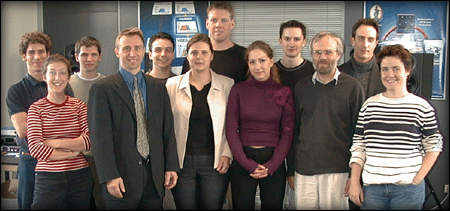
\includegraphics[width=12cm]{figures/equipe.png}\\
    \caption{L'equipe de GENESIS (avec deux stagiaires).}
    \label{equipe}
\end{figure}

GENESIS repose sur une {\'e}quipe de 10 salari{\'e}s. Sa partie recherche,
d{\'e}veloppement et production s'appuie sur des sp{\'e}cialistes dans 4
domaines de comp{\'e}tence :\\

\begin{itemize}
    \item Analyse et synth{\`e}se de son, transformation et traitement du signal
          audionum{\'e}rique.\\

    \item Simulation d'environnement sonore en trois dimensions, spatialisation
          des sources virtuelles.\\

    \item Psychoacoustique - {\'e}tude quantitative et qualitative de la perception
          et de la sensation auditive.\\

    \item Conception et r{\'e}alisation de syst{\`e}mes audionum{\'e}riques, Informatique,
          {\'e}lectronique analogique et num{\'e}rique, industrialisation, production.\\
\end{itemize}

Son savoir-faire est cultiv{\'e} et approfondi par une collaboration
permanente avec des centres de recherches, en particulier avec :\\

\begin{itemize}
    \item L'IRCAM (Institut de Recherche et Coordination Acoustique/Musique)
          {\`a} Paris.\\
    \item Le Laboratoire de M{\'e}canique et d'Acoustique (LMA) du CNRS {\`a} Marseille
          (Equipes Psychoacoustique et Informatique Musicale).\\
\end{itemize}

De plus, elle accueille dans son {\'e}quipe trois {\'e}tudiants effectuant
leur th{\`e}se, ce qui renforce son potentiel en recherche et d{\'e}veloppement.\\

\begin{figure}[h]
    \centering
    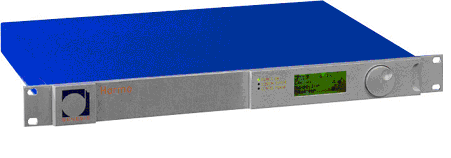
\includegraphics[width=12cm]{figures/harmo.png}\\
    \caption{L'Harmo.}
    \label{harmo}
\end{figure}

Les principales r{\'e}alisations de la soci{\'e}t{\'e} GENESIS sont :\\

\begin{itemize}
    \item l'environnement sonore du simulateur de vol pour les pilotes du
    SuperPuma (client Eurocopter),\\
    \item une {\'e}tude sur les bruits de circulation routi{\`e}re et
    ferroviaire (minist{\`e}re des transports et de l'{\'e}quipement,
    minist{\`e}re de l'environnement),\\
    \item une machine d{\'e}di{\'e}e , l'Harmo (fig. \ref{harmo}),
    permettant l'harmonisation \footnote{changement de
    la dur{\'e}e d'un son en modifiant le moins possible son timbre,
    sa hauteur...} en temps r{\'e}el de bandes sons. GENESIS a re\c{c}u
    le prix de l'innovation technologique Satisfecit pour ce
    produit lors de sa participation au SATIS (octobre 2001).\\
\end{itemize}

Enfin, GENESIS a su gagner la confiance d'importants groupes
industriels pour des {\'e}tudes ou des simulations d'environnements
sonores; on peut citer notamment P.S.A., Michelin, la S.N.C.F.,
Renault...


\chapter{Notions de psychoacoustique}
\label{theorie}
La psychoacoustique est la branche de l'acoustique qui {\'e}tudie la
perception des sons par l'homme. Il s'agit donc d'{\'e}tudier les
relations entre les stimuli sonores et les sensations, voir
l'absence de sensations, qu'ils provoquent chez l'auditeur. Ainsi
il sera possible de simplifier un son de mani{\`e}re {\`a} ne garder que
ses composantes pertinentes, c'est {\`a} dire vraiment entendues par
l'oreille. Une telle simplification peut servir pour de la
compression audio (comme dans le standard MP3 par exemple), ou
bien comme cela nous int{\'e}resse pour la synth{\`e}se de son lorsque le
synth{\'e}tiseur a une puissance de calcul limit{\'e}e.\\

Il faut tout de m{\^e}me garder {\`a} l'esprit que la plupart des
r{\'e}sultats de la psychoacoustique ont {\'e}t{\'e} d{\'e}termin{\'e}s
exp{\'e}rimentalement. De plus, ces r{\'e}sultats sont valables pour un
auditeur moyen, c'est {\`a} dire un sujet n'ayant pas de probl{\`e}me
d'ou{\"\i}e, mais qui n'a pas non plus une acuit{\'e} auditive entra{\^\i}n{\'e}e.
En effet, les ph{\'e}nom{\`e}nes psychoacoustiques sont en grande partie
dus {\`a} la physiologie de l'oreille qui elle-m{\^e}me varie d'un sujet {\`a}
l'autre. Ainsi, une adaptation des r{\'e}sultats en fonction du sujet
cible peut {\^e}tre envisageable, par exemple l'utilisation des
concepts psychoacoustiques ne sera pas la m{\^e}me suivant que la
cible est constitu{\'e}e de personnes {\^a}g{\'e}es ou de musiciens
confirm{\'e}s.\\

Nous allons donc voir au cours de ce chapitre les quelques
principes th{\'e}oriques sur lesquels s'appuie la bo{\^\i}te {\`a} outils
d{\'e}velopp{\'e}e.\\


\newpage
\section{Courbes d'isosonie}
Courbes reliant la sensation de force du signal sonore sur
l'auditeur, exprim{\'e}e en sones, et l'intensit{\'e} acoustique r{\'e}elle,
mesur{\'e}e en d{\'e}cibels SPL \footnote{Le dB SPL (pour Sound Pressure
Level) quantifie l'intensit{\'e} acoustique d'un stimulus sonore. Il
est d{\'e}finie par $ I_{SPL} = 20 * \log _{10} \( \frac{P}{P_{0}} \)
$ o{\`u} $P_{0}$ repr{\'e}sente est la r{\'e}f{\'e}rence de 20 $\mu$ Pa. Ainsi un
niveau de 0 dB SPL correspond {\`a} un signal {\`a} la limite de l'audition {\`a} 1 kHz.}.\\

\begin{figure}[h]
    \bigskip
    \centering
    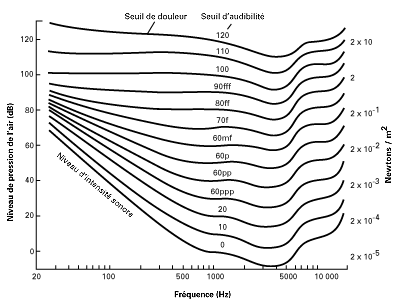
\includegraphics[width=12cm]{figures/isosonie.png}\\
    \caption{Courbes d'isosonie.}
    \label{isosonie}
    \bigskip
\end{figure}

Ces courbes, d{\'e}termin{\'e}es exp{\'e}rimentalement au cours des ann{\'e}es
trente \footnote{H. Fletcher et W. Munson, "Relation between
loudness and masking", \emph{J. Acoust. Soc. Amer.}, vol. 9, pp.
1-10, 1937.}, permettent d'{\'e}tablir la sensation de perception
{\'e}gale d'une intensit{\'e} acoustique donn{\'e}e, et cela pour l'ensemble
du spectre fr{\'e}quentiel audible. Elles sont extr{\^e}mement utiles
lorsqu'il s'agit de d{\'e}terminer les r{\'e}gions spectrales
significatives sur le plan perceptif lors d'op{\'e}rations d'encodage
et de compression de signaux audio-num{\'e}riques.\\

En particulier, la courbe du seuil absolue d'audition se place
pour des signaux sonores {\`a} la limite de la sensation de
perception. Une approximation possible \footnote{E. Terhardt,
"Calculating virtual pitch", \emph{Hearing res.}, vol. 1, pp.
155-182, 1979.} de ce seuil en fonction de la fr{\'e}quence est :
$$ S(f) = 3.64*f^{-0.8} - 6.5*e^{-0.6*(f-3.3)^{2}} + 10^{-3}*f^{4} $$
o{\`u} f est en kHz et S en dB SPL.


\newpage
\section{Bandes critiques}
Pour une fr{\'e}quence centrale donn{\'e}e, la bande critique est la plus
petite largeur spectrale pour laquelle une m{\^e}me zone de la
membrane basilaire est excit{\'e}e. En effet, lorsque une onde sonore
arrive au pavillon de l'oreille, elle est transmise par la cha{\^\i}ne
des osselets (non repr{\'e}sent{\'e}e figure \ref{cochlee}) {\`a} l'oreille
interne. Cette derni{\`e}re se compose essentiellement de la cochl{\'e}e
(ou lima\c{c}on en raison de sa forme). Celle-ci est constitu{\'e}e de
deux canaux, les rampes vestibulaire et tympanique, s{\'e}par{\'e}s par la
la cloison cochl{\'e}aire. Cette cloison comprend la membrane de
Reissner, la membrane tectoriale, la membrane basilaire ainsi que
l'organe de Cortie pris entre ces deux derni{\`e}res. La vibration
sonore engendre des ventres d'onde le long de la membrane
basilaire {\`a} des positions sp{\'e}cifiques de sa fr{\'e}quence. Or l'organe
de Cortie qui repose sur la membrane basilaire, est constitu{\'e}e de
cellules cili{\'e}es au contact desquelles prennent naissance les
fibres du nerf auditif.\\

\begin{figure}[h]
    \bigskip
    \centering
    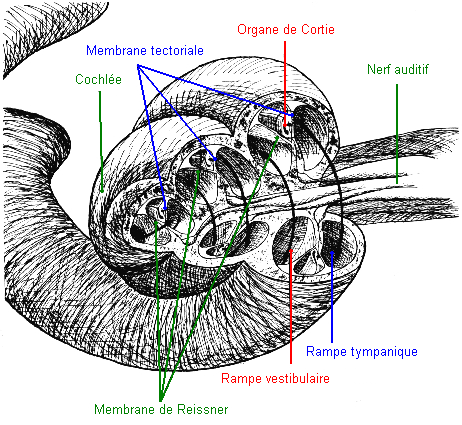
\includegraphics[width=12cm]{figures/cochlee.png}\\
    \caption{Coupe de la cochl{\'e}e.}
    \label{cochlee}
    \bigskip
\end{figure}

C'est l'espacement de ces cellules cili{\'e}es le long de la membrane
basilaire qui engendre le ph{\'e}nom{\`e}ne des bandes critiques. En effet
chaque r{\'e}cepteur nerveux se trouve accord{\'e} {\`a} une certaine
fr{\'e}quence due {\`a} sa position sur la membrane basilaire. Ainsi,
l'oreille effectue une transformation fr{\'e}quences/positions, et
c'est bien une information de position qui est transmise au
cerveau par le nerf auditif.\\

En cons{\'e}quence d'une telle transformation, le fonctionnement de
l'oreille interne s'apparente {\`a} celui d'un banc de filtres
passe-bandes {\`a} fort taux de recouvrement \footnote{i.e. les bandes
passantes des filtres se chevauchent.}, de plus la r{\'e}ponse en
fr{\'e}quence de chacun de ces filtres est asym{\'e}trique et leur
bande-passante d{\'e}pend de la fr{\'e}quence centrale \footnote{D. D.
Greenwood, "Critical bandwith and the frequency coordinates of the
basilar membrane", \emph{J. Acoust. Soc. Amer.}, pp. 1344-1356,
Oct. 1961.}, la bande-critique correspondrait {\`a} la largeur de la
bande-passante. En cons{\'e}quence, si deux fr{\'e}quences pures
appartenant {\`a} la m{\^e}me bande critique se pr{\'e}sentent au m{\^e}me instant
{\`a} l'oreille, il est possible que l'auditeur n'en per\c{c}oive qu'une.
Ainsi, une {\'e}chelle des fr{\'e}quences rendant compte de ces ph{\'e}nom{\`e}nes
a {\'e}t{\'e} invent{\'e}e, le Bark, et elle sera utilis{\'e}e avantageusement {\`a}
la place de l'{\'e}chelle de Hertz lorsqu'il est question de
perception humaine de signaux sonores. Un bark est d{\'e}fini comme la
largeur d'une bande critique, donc dans l'{\'e}chelle
de Bark les filtres sont de bande-passante constante.\\

\begin{figure}[h]
\bigskip
\begin{center}
    \begin{tabular}{|c|c||c|c||c|c|}
        \hline
        Bark &   Hertz   &   Bark    &   Hertz   &   Bark    &   Hertz\\
        \hline
        1    &   101     &   9       &   1079    &   17      &   3822\\
        2    &   204     &   10      &   1255    &   18      &   4554\\
        3    &   308     &   11      &   1456    &   19      &   5411\\
        4    &   417     &   12      &   1690    &   20      &   6414\\
        5    &   530     &   13      &   1968    &   21      &   7617\\
        6    &   651     &   14      &   2302    &   22      &   9166\\
        7    &   781     &   15      &   2711    &   23      &   11414\\
        8    &   922     &   16      &   3211    &   24      &   15405\\
        \hline
    \end{tabular}
\end{center}
\caption{Equivalence Bark/Hertz.}
\label{tabbark2hz}
\bigskip
\end{figure}

Pour un auditeur moyen, la largeur (en Hz) de bande critique en
fonction de la fr{\'e}quence centrale peut {\^e}tre estim{\'e}e par :
$$ BP_{crit}(f) = 25 + 75*\[ 1 + 1.4*\( \frac{f}{1000} \)^{2} \]^{0.69} $$
de plus, la formule :
$$ B(f) = 13 * \arctan\(7.6*10^{-4}*f\) + 3.5*\arctan\[\(\frac{f}{7500}\)^{2}\]$$
est souvent utilis{\'e}e pour convertir les Hertz en Bark
\footnote{Ces deux formules sont tir{\'e}es de: E. Zwicker et H.
Fastl, "Psychoacoustics facts en models", 1990.}.


\newpage
\section{Masquage fr{\'e}quentiel}
On parle de masquage lorsque une composante sonore est rendue
inaudible {\`a} cause de la pr{\'e}sence d'une autre composante. Le
masquage fr{\'e}quentiel, ou masquage simultan{\'e}, peut arriver lorsque
deux stimuli sonores ou plus sont pr{\'e}sent{\'e}s au syst{\`e}me auditif.
Plus pr{\'e}cis{\'e}ment, un signal sonore puissant peut engendrer une
excitation de la membrane basilaire suffisamment forte pour
emp{\^e}cher l'audition d'un signal plus faible situ{\'e} dans la m{\^e}me
bande critique. Malgr{\'e} le fait que les spectres de signaux audios
r{\'e}els peuvent g{\'e}n{\'e}rer une infinit{\'e} de scenarii de masquage
diff{\'e}rents, il est commun de s{\'e}parer ce ph{\'e}nom{\`e}ne en trois
probl{\`e}mes distincts et g{\'e}n{\'e}riques, facilitant ainsi son
exploitation dans des algorithmes audio-num{\'e}riques.\\

    \newpage
    \subsection{Masquage d'un ton par un autre ton}

    \begin{figure}[h]
        \centering
        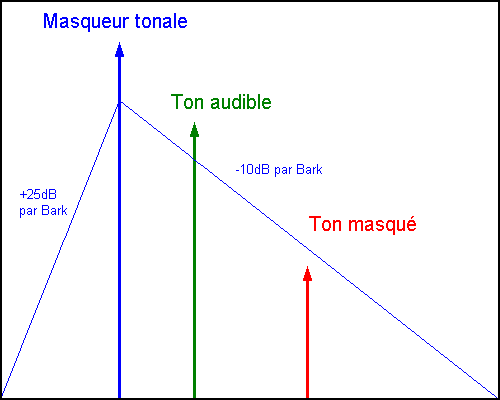
\includegraphics[width=12cm]{figures/masquage_tt.png}\\
        \caption{Ton masqu{\'e} par un ton.}
        \label{masquage_tt}
    \end{figure}

    Dans le cas d'interaction de deux signaux purement sinuso{\"\i}daux,
    on consid{\'e}rera qu'un ton est inaudible si il est situ{\'e} en
    dessous de la courbe de masquage (cf figure \ref{masquage_tt})
    induite par la fr{\'e}quence ayant localement le plus d'{\'e}nergie.
    Il est {\`a} noter que cette courbe ne s'{\'e}tale pas uniquement sur
    la bande critique de la fr{\'e}quence consid{\'e}r{\'e}e.


    \newpage
    \subsection{Masquage d'un ton par un bruit}
    Il peut arriver qu'un ton soit masqu{\'e} par le bruit de fond
    situ{\'e} dans la m{\^e}me bande critique. Cela arrive lorsque
    l'{\'e}nergie moyenne de la bande critique consid{\'e}r{\'e}e est
    sup{\'e}rieure d'au moins 4 dB {\`a} l'{\'e}nergie du signal sinuso{\"\i}dal.
    Une {\'e}tude de ce ph{\'e}nom{\`e}ne pourra {\^e}tre trouv{\'e}e dans [R.
    Hellman, "Assymetry of maskink between noise and tone",
    Percept. Psychphys, vol. 11, pp. 241-246, 1972].

    \begin{figure}[h]
        \centering
        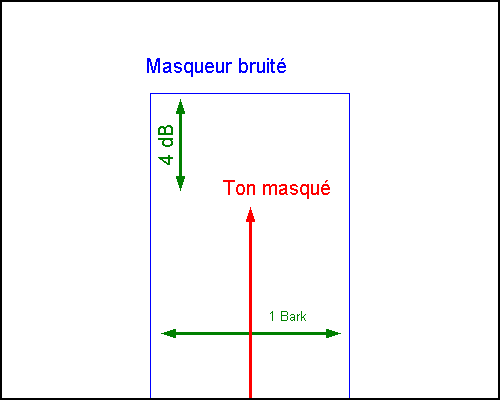
\includegraphics[width=12cm]{figures/masquage_tb.png}\\
        \caption{Ton masqu{\'e} par une bande de bruit.}
        \label{masquage_tb}
    \end{figure}


    \newpage
    \subsection{Masquage d'un bruit par un ton}
    La situation inverse est {\'e}galement possible. C'est {\`a} dire
    qu'un ton masquera le bruit de fond de sa bande critique si
    l'{\'e}nergie du signal pure est sup{\'e}rieure d'au moins 24 dB {\`a}
    l'{\'e}nergie moyenne de la bande critique consid{\'e}r{\'e}e. Une {\'e}tude
    compl{\`e}te de ce cas ainsi que du cas o{\`u} un ton masque un autre
    ton pourra {\^e}tre trouv{\'e}e dans [B. C. J. Moore, J. I.
    Alc\'{a}ntara et T. Dau, "Masking patterns for sinusoidal and
    narrow-band noise maskers", \emph{J. Acoust. Soc. Amer.}, vol.
    104, no. 2.1, pp 1023-1038, jan. 1998].\\

    \begin{figure}[h]
        \centering
        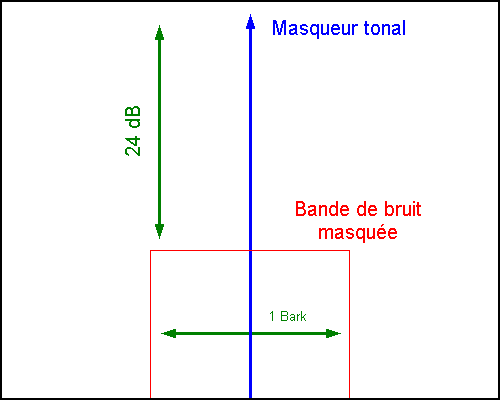
\includegraphics[width=12cm]{figures/masquage_bt.png}\\
        \caption{Bande de bruit masqu{\'e}e par un ton.}
        \label{masquage_bt}
    \end{figure}

    On remarque une dissym{\'e}trie entre ces deux derniers
    ph{\'e}nom{\`e}nes. Elle rend compte du fait que l'oreille humaine
    distingue plus facilement un signal sinuso{\"\i}dal noy{\'e} dans du
    bruit que l'inverse.


\chapter{Manuel d'utilisation de la bo{\^\i}te {\`a} outils}
\label{manuel}
%%%%%%%%%%%%%%%%%%%%%%%%    PRESENTATION    %%%%%%%%%%%%%%%%%%%%%%%%
\section*{Pr{\'e}sentation}
\addcontentsline{toc}{section}{Pr{\'e}sentation}

    Ce manuel a pour but d'expliquer le fonctionnement et l'utilisation
    des fonctions \matlab contenues dans le r{\'e}pertoire "{\it SoundToolBox}".\\

    A noter tout de m{\^e}me qu'une aide en ligne est accessible sous
    \matlabv il suffit de taper "{\tt help {\bf nom\_de\_commande}}" {\`a} la
    ligne de commande pour voir l'aide sur {\tt {\bf nom\_de\_commande}},
    ou "{\tt help soundtoolbox}" pour voir l'ensemble des fonctions de
    la boite {\`a} outils accompagn{\'e} d'un descriptif rapide de chacune
    d'elles. De plus les codes sources ont {\'e}t{\'e} largement comment{\'e}s.\\

    Le but de cette boite {\`a} outils est d'aider {\`a} l'analyse de sons
    {\color{red} \textbf{STATIONNAIRES}}, d'automatiser un certains
    nombres de proc{\'e}dures, et enfin d'extraire des composantes
    pertinentes au sens psychoacoustique en vu de leur synth{\`e}se en
    temps r{\'e}el.\\

    Les fonctions {\'e}crites ont {\'e}t{\'e} class{\'e}es par cat{\'e}gories. Chaque
    chapitre correspondant {\`a} une cat{\'e}gorie particuli{\`e}re:

    \begin{enumerate}
        \item fonctions ayant uniquement rapport {\`a} des notions
        psychoacoustiques; (page \pageref{secpsycho})

        \item fonctions effectuant des traitements "classiques" en
        th{\'e}orie du signal; (page \pageref{secclassiques})

        \item fonctions d'automatisation pour l'analyse de
        caract{\'e}ristiques spectrales; (page \pageref{secanalyses})

        \item fonctions pour extraire les composantes pertinentes
        d'un son complexe en vu de sa simplification; (page
        \pageref{secsimplification})

        \item fonctions annexes de sauvegarde, de pr{\'e}paration de
        sons... (page \pageref{secannexes})
    \end{enumerate}

    Enfin, le dernier chapitre explique comment installer et
    utiliser cette boite {\`a} outils avec \matlab (page
    \pageref{secutilisation}).\\

    \bigskip
    \textbf{Conventions typographiques :}\\
    \begin{center}
           {\tt [ out1, out2 ] = cmd( in1 [, in2, in3 ] ) }
    \end{center}
    est la commande \matlab {\tt cmd} d'arguments d'entr{\'e}e {\tt in1,
    in2} et {\tt in3} dont les deux derniers sont optionnels;
    d'arguments de sortie {\tt out1} et {\tt out2}. Si le
    comportement de la fonction est chang{\'e} lorsqu'il n'y a pas
    d'argument de sortie, cela est pr{\'e}cis{\'e}.

%%%%%%%%%%%%%%%%%%%%%%%%%%%%%%%%%%%%%%%%%%%%%%%%%%%%%%%%%%%%%%%%%%%%

%%%%%%%%%%%%%%%%%%%%%%%%%    DESCRIPTIF    %%%%%%%%%%%%%%%%%%%%%%%%%
\section*{Descriptif rapide des fonctions}
\addcontentsline{toc}{section}{Descriptif rapide des fonctions}

\begin{itemize}
\bigskip
\item Fonctions psychoacoustiques :
    \begin{description}
        \item[\textbf{\tt bark2hz.........}]conversion Bark $\rightarrow$ Hertz.
        \item[\textbf{\tt critical\_band...}]Calcul des fr{\'e}quences limites d'une fen{\^e}tre fr{\'e}quentielle.
        \item[\textbf{\tt hz2bark.........}]Conversion Hertz $\rightarrow$ Bark.
        \item[\textbf{\tt threshold.......}]Seuil d'audition en fonction de la fr{\'e}quence.
    \end{description}

\bigskip
\item Fonctions classiques de traitement de signaux :
    \begin{description}
        \item[\textbf{\tt dirac\_sequence...}]Generation d'un peigne de dirac de largeurs fixes.
        \item[\textbf{\tt get\_lpsd.........}]Calcul et affichage de la \dsp d'un son en dB.
        \item[\textbf{\tt get\_psd..........}]Calcul et affichage de la \dsp d'un son.
        \item[\textbf{\tt normalize........}]Normalisation d'un signal temporel en {\'e}nergie.
    \end{description}

\bigskip
\item Fonctions d'analyse de signaux num{\'e}riques :
    \begin{description}
        \item[\textbf{\tt analyse\_harm.....}]Automatisation de {\tt mean\_harmonics}.
        \item[\textbf{\tt get\_all\_tones....}]D{\'e}tection des partiels d'un son.
        \item[\textbf{\tt get\_funds........}]Recherche des fr{\'e}quences fondamentales parmi un tableau de fr{\'e}quences.
        \item[\textbf{\tt get\_harmonics....}]D{\'e}tection de suites harmoniques d'un son.
        \item[\textbf{\tt get\_harm\_dir.....}]D{\'e}tection et sauvegarde de suites harmoniques des sons d'un repertoire.
        \item[\textbf{\tt mean\_harmonics...}]D{\'e}tection de suites harmoniques extrait de plusieurs fichiers wave.
    \end{description}

\bigskip
\item Fonctions permettant la simplification de sons complexes :
    \begin{description}
        \item[\textbf{\tt analyse\_pert........}]Automatisation de {\tt mean\_pertinents}.
        \item[\textbf{\tt analyse\_pert\_harm...}]Automatisation de {\tt mean\_pert\_harm}.
        \item[\textbf{\tt clone\_wave..........}]Copie d'un fichier wave gr{\^a}ce {\`a} {\tt mean\_pertinents}.
        \item[\textbf{\tt decimation..........}]Proc{\'e}dure de decimation des composantes tonales d'un son.
        \item[\textbf{\tt get\_noise\_band......}]Evaluation des niveaux de bandes de bruit equivalent a une \dsp.
        \item[\textbf{\tt get\_pertinents......}]Extraction des composantes pertinentes d'un son.
        \item[\textbf{\tt get\_pert\_dir........}]Processus d'extraction appliqu{\'e} {\`a} tous les sons d'un r{\'e}pertoire.
        \item[\textbf{\tt get\_pert\_harm.......}]Extraction des s{\'e}quences harmoniques pertinentes.
        \item[\textbf{\tt mean\_pertinents.....}]Extraction et moyenne des composantes pertinentes de sons.
        \item[\textbf{\tt mean\_pert\_harm......}]Extraction et moyenne des s{\'e}quences harmoniques pertinentes.
        \item[\textbf{\tt synthetize..........}]Synth{\`e}se d'un son {\`a} partir de ses composantes pertinentes.
    \end{description}

\bigskip
\item Fonctions diverses :
    \begin{description}
        \item[\textbf{\tt cell2file.......}]Sauvegarde d'un tableau de cellules dans un fichier texte.
        \item[\textbf{\tt cell\_fusion.....}]Fusion de deux tableaux de cellules repr{\'e}sentant des s{\'e}quences harmoniques.
        \item[\textbf{\tt cell\_sort.......}]Tri par ordre croissant des fr{\'e}quences fondamentales d'un tableau de cellules.
        \item[\textbf{\tt cut\_wavfile.....}]D{\'e}coupage d'un fichier wave en plusieurs fichiers.
        \item[\textbf{\tt fusion..........}]Fusion de deux tableaux d'une m{\^e}me s{\'e}quence harmonique en un seul.
        \item[\textbf{\tt get\_all\_dir.....}]R{\'e}cup{\'e}ration des noms des sous r{\'e}pertoires.
        \item[\textbf{\tt get\_all\_files...}]R{\'e}cup{\'e}ration de tous les noms de fichier contenant une cha{\^\i}ne de caract{\`e}res.
        \item[\textbf{\tt insertion.......}]Insertion d'un tableau de 25 niveaux de bruit dans un fichier.
        \item[\textbf{\tt noises2file.....}]Sauvegarde d'un tableau dans un fichier.
        \item[\textbf{\tt now2str.........}]Affichage de la date et de l'heure.
        \item[\textbf{\tt prepare\_dir.....}]Preparation d'un r{\'e}pertoire de fichiers wave en vu de leur traitement.
        \item[\textbf{\tt sec2hour........}]Conversion d'un nombre de secondes en heures, minutes, secondes, millisecondes.
        \item[\textbf{\tt tones2file......}]Sauvegarde d'un tableau de fr{\'e}quences et d'amplitudes dans un fichier.
    \end{description}
\end{itemize}

%%%%%%%%%%%%%%%%%%%%%%%%  PSYCHOACOUSTIQUE  %%%%%%%%%%%%%%%%%%%%%%%%
\newpage
\section{Fonctions psycho-acoustiques}
\label{secpsycho}

%    \newpage
    \bigskip
    \subsection{Bark2hz}
    \label{bark2hz}
    La fonction {\tt F$_{\tt Hz}$ = bark2hz( F$_{\tt bark}$ )}
    convertie {\tt F$_{\tt bark}$} repr{\'e}sentant une valeur ou
    un tableau de valeurs en Bark, en son (ses) correspondant(s)
    en Hertz. Pour ce faire, la valeur en Hertz est approch{\'e}e gr{\^a}ce
    {\`a} la formule :

    $$ {\tt F_{app}} = 1960 * \frac{0.53 + {\tt F_{bark}}}{26.28 - {\tt F_{bark}}}
    $$

    \noindent puis la fonction \matlab {\tt fsolve} (toolbox optim)
    est utilis{\'e}e pour r{\'e}soudre l'{\'e}quation :

    $$ {\tt hz2bark}({\tt F_{Hz}}) - {\tt F_{bark}} = 0 $$

    \noindent la valeur {\tt F$_{\tt app}$} servant de base de
    recherche de la solution pour {\tt fsolve}. La figure
    \ref{tabbark2hz} montre l'{\'e}quivalent en Hertz des fr{\'e}quences
    1 {\`a} 24 Bark.\\


    \newpage
%    \bigskip
    \subsection{Critical\_band}
    \label{criticalband}
    La fonction {\tt [ F$_{\tt down}$, F$_{\tt up}$ ] = critical\_band( F, bw )}
    calcule les fr{\'e}quences limites basse ({\tt F$_{\tt down}$})
    et haute ({\tt F$_{\tt up}$}) en hertz d'une fen{\^e}tre de largeur
    {\tt bw} bark centr{\'e}e g{\'e}om{\'e}triquement sur la fr{\'e}quence {\tt F}
    en Hertz. Nous avons donc les relations suivantes :

    $$ {\tt F} = \sqrt{ {\tt F_{down}} * {\tt F_{up}} } $$
    \begin{center} et \end{center}
    $$ {\tt F_{up}} - {\tt F_{down}} = {\tt bw}\:(\mbox{ en Hz })$$.

    Pour acc{\'e}l{\'e}rer le traitement, une simplification a {\'e}t{\'e}
    effectu{\'e}e, si bien qu'au del{\`a} de 12 kHz, la fen{\^e}tre ne fait
    plus la largeur sp{\'e}cifi{\'e}e ( {\`a} 15 kHz 0.75 bark de large alors
    pour 1 bark demand{\'e} ).\\

    \begin{verbatim}
        >> [F_down,F_up]=critical_band(440,1);...
                hz2bark(F_up)-hz2bark(F_down)

        ans =

           1.0128

        >> [F_down,F_up]=critical_band(12e3,1);...
                hz2bark(F_up)-hz2bark(F_down)

        ans =

          0.9294
    \end{verbatim}


    \newpage
%    \bigskip
    \subsection{Hz2bark}
    \label{hz2bark}
    La fonction {\tt F$_{\tt bark}$ = hz2bark( F$_{\tt Hz}$ )}
    convertie la (les) fr{\'e}quence(s) {\tt F$_{\tt Hz}$} en bark
    selon la formule :

    $$ {\tt F_{bark}} =
                13 * \arctan{({7.6*10^{-4}})*{\tt F_{Hz}}}
                                 +
            3.5 * \arctan{\( \frac{\tt F_{Hz}}{7500} \) }^2$$

    La figure \ref{fighz2bark} montre la correspondance entre
    l'{\'e}chelle des hertz et celle des bark.\\

    \medskip
    \begin{figure}[h]
      \centering
      {\tt >> plot( 20:20000, hz2bark(20:20000) );\\
           >> grid on; xlabel('Hertz'); ylabel('Bark'); }\\
      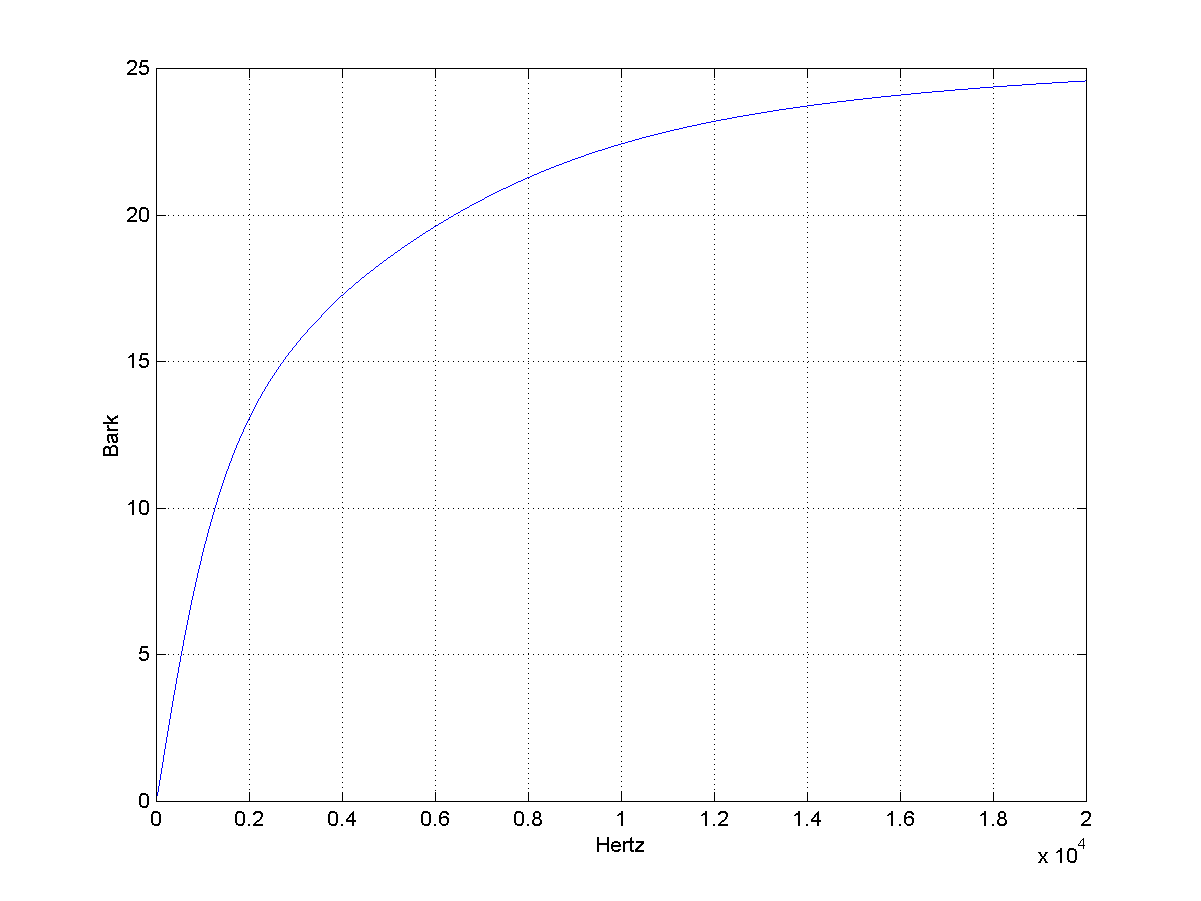
\includegraphics[width=12cm]{figures/hz2bark.png}\\
      \caption{Equivalence Hertz/Bark.}
      \label{fighz2bark}
    \end{figure}
    \medskip

    \newpage
%    \bigskip
    \subsection{Threshold}
    \label{threshold}
    La fonction {\tt pond{\'e}ration = threshold( F$_{\tt Hz}$ )} permet
    d'estimer la pond{\'e}ration due au seuil d'audition absolu gr{\^a}ce
    {\`a} la formule :

    $$ {\tt seuil_{dB}} = 3.64 * \( \frac{\tt F_{Hz}}{1000} \) ^{-0.8}
                      - 6.5*e^{-0.6*\( \frac{\tt F_{Hz}}{1000} - 3.3\)^2}
                         + 10^{-3}*\( \frac{\tt F_{Hz}}{1000}\)^4         $$

    Nous avons donc :
    $$ {\tt ponderation} = 10^\frac{\tt seuil_{dB}}{10} $$
    o{\`u} on divise par 10 puisque cette pond{\'e}ration s'appliquera {\`a}
    des niveaux {\'e}nerg{\'e}tiques.

    A noter que si l'argument de sortie n'est pas pr{\'e}cis{\'e},
    la fonction affiche le seuil en dB SPL comme le montre
    la figure \ref{figthreshold}.\\

    \medskip
    \begin{figure}[h]
      \centering
      {\tt >> threshold(20:20000)}\\
      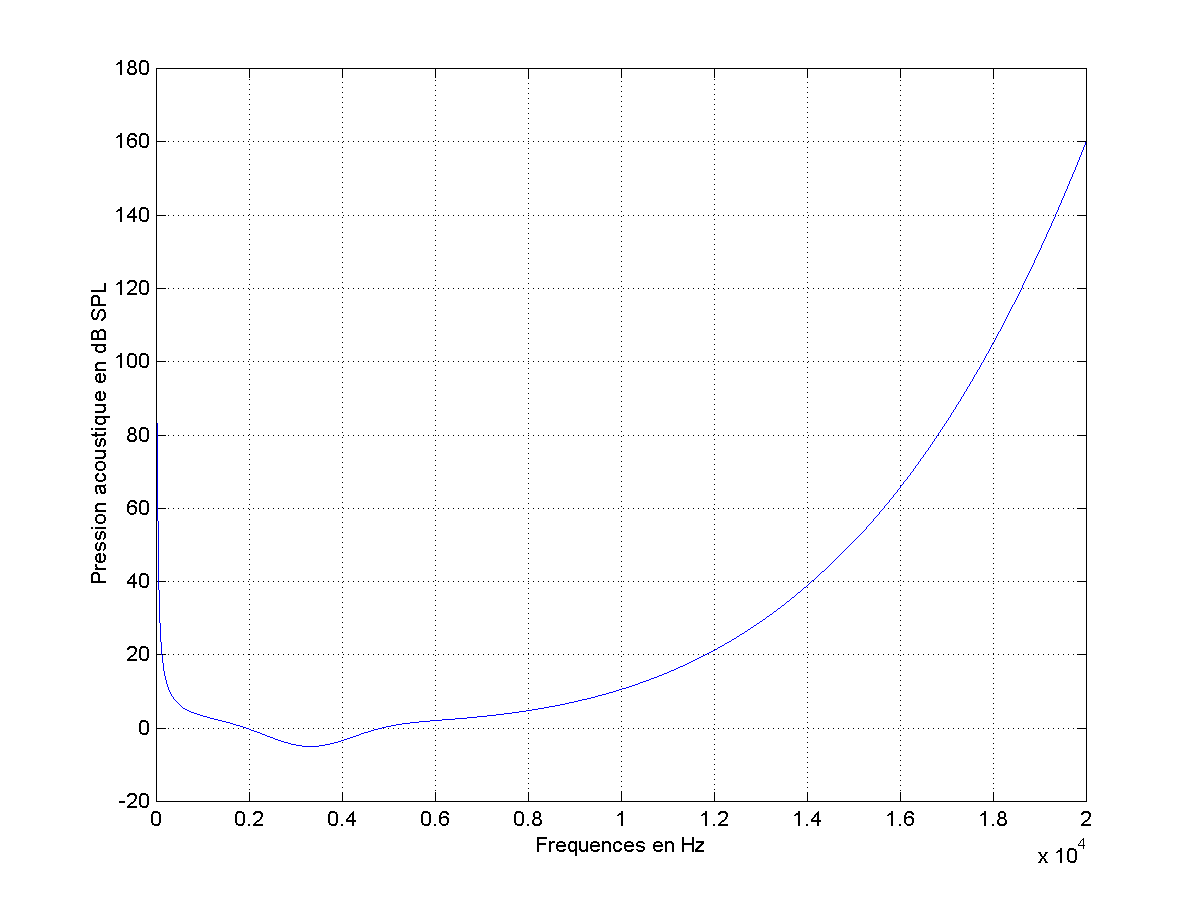
\includegraphics[width=12cm]{figures/threshold.png}\\
      \caption{Pression acoustique {\'e}quivalente au seuil d'audition.}
      \label{figthreshold}
    \end{figure}
    \medskip

%%%%%%%%%%%%%%%%%%%%%%%%%%%%%%%%%%%%%%%%%%%%%%%%%%%%%%%%%%%%%%%%%%%%


%%%%%%%%%%%%%%%%%%%%%%  FONCTIONS CLASSIQUES  %%%%%%%%%%%%%%%%%%%%%%
\newpage
\section{Fonctions classiques}
\label{secclassiques}


%    \newpage
    \bigskip
    \subsection{Dirac\_sequence}
    \label{diracsequence}
    {\tt sequ = dirac\_sequence( f0 [, nb, fs, len, wid ] )}
    g{\'e}n{\'e}re une s{\'e}quence de {\tt nb} portes de largeur {\tt wid} Hz,
    la s{\'e}quence fait {\tt len} {\'e}chantillons fr{\'e}quentiels, la
    fr{\'e}quence d'{\'e}chantillonnage {\'e}tant de {\tt fs}, la distance
    entre le centre de chacune des portes est de {\tt f0} Hz. Les
    valeurs par d{\'e}faut sont {\tt nb = 0}, {\tt fs = 44100}, {\tt
    len = 32768} et {\tt wid = 4}.\\

    Si {\tt nb} est {\'e}gal {\`a} 0, le nombres de portes est maximal, et
    c'est le cas par d{\'e}faut. Enfin si l'argument de sortie n'est
    pas pr{\'e}cis{\'e}, la s{\'e}quence est affich{\'e}e (figure \ref{figdirac}),
    cela peut {\'e}ventuellement servir pour les phases de test.\\

    \medskip
    \begin{figure}[h]
      \centering
      {\tt >> dirac\_sequence(2500)}\\
      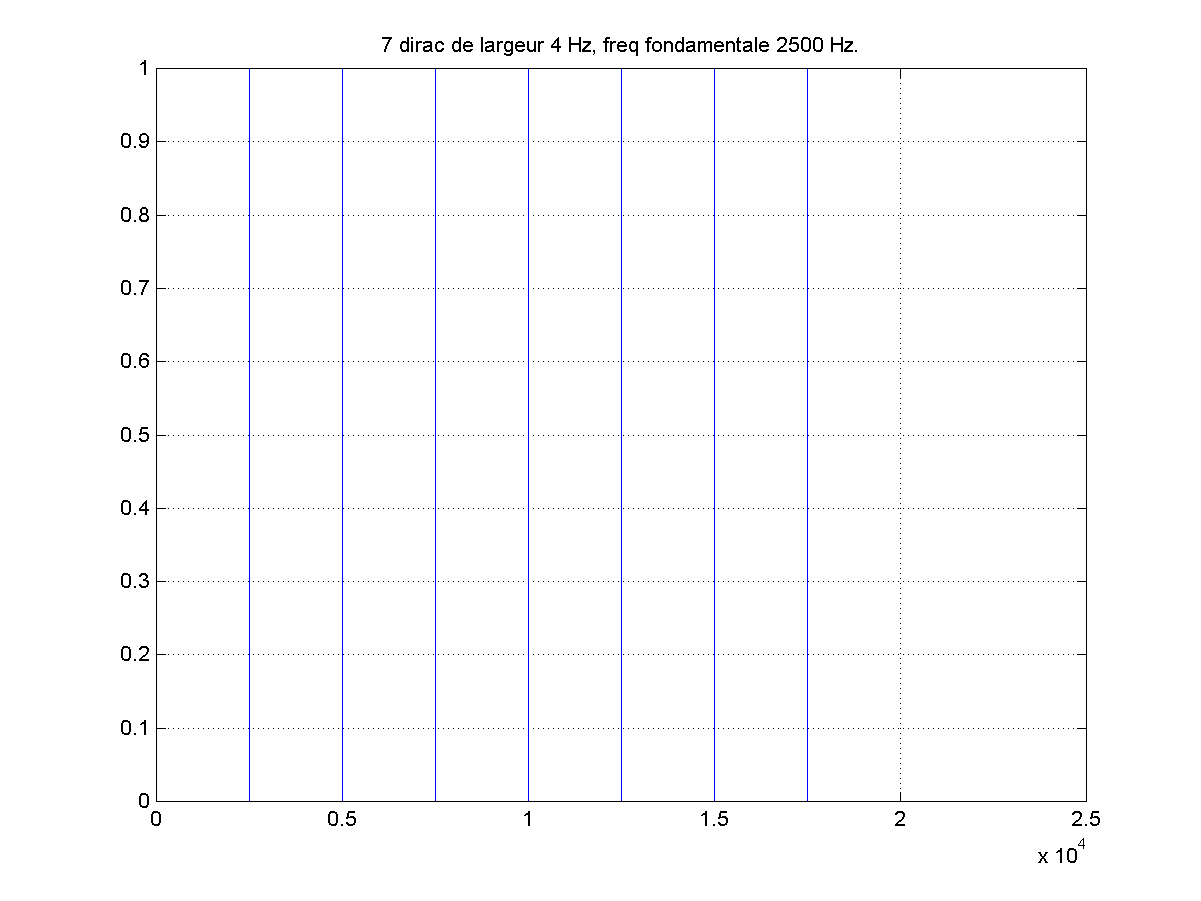
\includegraphics[width=12cm]{figures/dirac.png}\\
      \caption{S{\'e}quence de dirac.}
      \label{figdirac}
    \end{figure}
    \medskip

    \newpage
%    \bigskip
    \subsection{Get\_psd et get\_lpsd}
    \label{getpsd}
    {\tt dsp = get\_psd( sig )} et {\tt dspl = get\_lpsd( sig )}
    calculent respectivement la densit{\'e} spectrale de puissance
    en lin{\'e}aire et en dB {\`a} partir du tableau de valeurs {\tt sig}.
    Ces fonctions peuvent {\'e}galement {\^e}tre utilis{\'e}es sous la forme:
    \begin{center}
    {\tt dsp = get\_psd( wavfile )} et {\tt dspl = get\_lpsd( wavfile )},
    \end{center}
    o{\`u} l'argument {\tt wavfile} est une cha{\^\i}ne de caract{\`e}res
    contenant le nom d'un fichier au format wave. L'argument de sortie {\tt dsp} sera
    la \dsp regroupant les fr{\'e}quences n{\'e}gatives et positives, alors
    que {\tt dspl} ne contient que les fr{\'e}quences positives.

    Si l'argument de sortie n'est pas pr{\'e}cis{\'e}, le r{\'e}sultat
    du calcul est affich{\'e} (figure \ref{figpsd}), il est alors possible
    d'ajouter la fr{\'e}quence d'{\'e}chantillonnage {\tt fs} pour avoir l'axe des abscisses en hertz
    et un dernier argument pr{\'e}cisant le num{\'e}ro de figure,
    ce qui peut {\^e}tre pratique lorsque l'on veut afficher
    plusieurs densit{\'e}s spectrales de puissance {\`a} la suite.\\

    Enfin, pr{\'e}cisons que le zero-padding est effectu{\'e} {\`a} l'int{\'e}rieur
    de la fonction mais pas le fen{\^e}trage. Le nombre d'{\'e}chantillons
    du signal sur lequel est appliqu{\'e} la transform{\'e}e de Fourier
    rapide est port{\'e} {\`a} $2^{17} = 131072$ {\'e}chantillons, ou si le
    nombre d'origine est sup{\'e}rieur, {\`a} la puissance de 2
    strictement sup{\'e}rieure. Ceci permet {\`a} la fois de gagner en
    pr{\'e}cision fr{\'e}quentielle (nombre d'{\'e}chantillons) et en
    pr{\'e}cision sur les niveaux (nombre de z{\'e}ro {\`a} la suite du signal
    utile)\\

    \medskip
    \begin{figure}[h]
      \centering
      {\tt >> get\_lpsd('9\_vh\_100\_2200ft.wav')}\\
      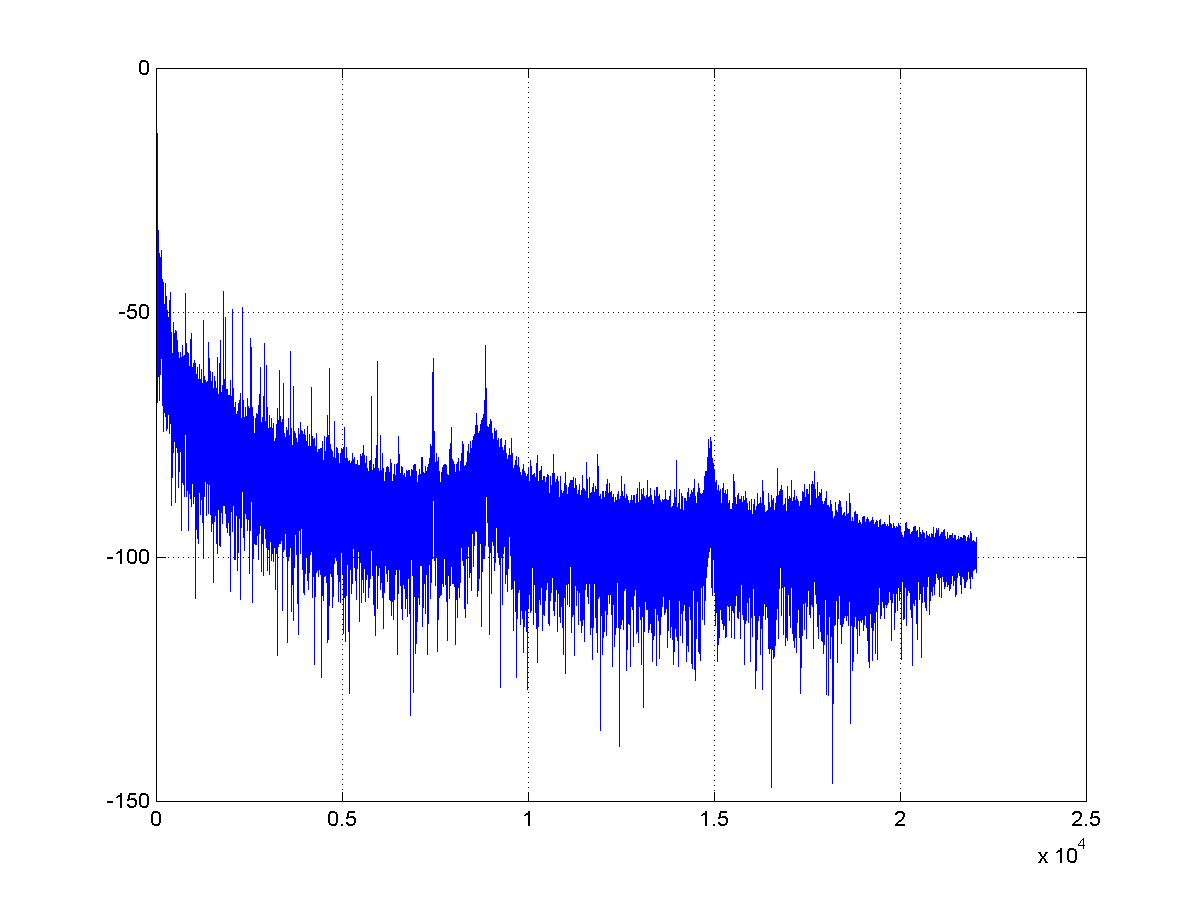
\includegraphics[width=12cm]{figures/lpsd.png}\\
      \caption{Affichage typique de la fonction {\tt get\_lpsd}.}
      \label{figpsd}
    \end{figure}
    \medskip


    \newpage
%    \bigskip
    \subsection{Normalize}
    \label{normalize}
    La fonction {\tt Y = normalize( X )} normalise le signal {\tt X}
    en puissance, nous avons donc :

    $$ {\tt Y} = \sqrt{ \frac{\tt N}{\sum_{{\tt n}=1}^{\tt N}{\tt x_n^2 }} } * {\tt X} $$
    et par construction :
    $$ \frac{1}{\tt N} \sum_{{\tt n}=1}^{\tt N}{\tt y_n^2} = 1 $$

    o{\`u} {\tt N} est le nombre d'{\'e}chantillons ${\tt x_n}$ du signal
    {\tt X} et les ${\tt y_n}$ sont les {\'e}chantillons du signal
    {\tt Y}.\\

    Un exemple d'utilisation sous \matlab : normalisation en
    puissance d'un signal sinuso{\"\i}dal de fr{\'e}quence 440 Hz, de 2048
    {\'e}chantillons : \\

    \begin{verbatim}
        >> X=sin(2*pi*440*(0:2047)/44100); sum( X.^2 )/2048

        ans =

          0.5014

        >> Y=normalize(X); sum( Y.^2 )/2048

        ans =

          1.0000
    \end{verbatim}

%%%%%%%%%%%%%%%%%%%%%%%%%%%%%%%%%%%%%%%%%%%%%%%%%%%%%%%%%%%%%%%%%%%%


%%%%%%%%%%%%%%%%%%%%%%%  FONCTIONS ANALYSES  %%%%%%%%%%%%%%%%%%%%%%%
\newpage
\section{Fonctions d'analyses}
\label{secanalyses}


    %\newpage
    \bigskip
    \subsection{Get\_all\_tones}
    \label{getalltones}
    La fonction
    \begin{center}
    {\tt [freq, peak, dsp] = get\_all\_tones( signal, fs [, thr, win ])}
    \end{center}
    permet d'extraire les fr{\'e}quences pures d'un
    son {\tt signal} {\'e}chantillonn{\'e} {\`a} {\tt fs} Hz. Pour ce faire,
    la \dsp du signal fen{\^e}tr{\'e} par {\tt win} (par d{\'e}faut {\tt win } est
    une fen{\^e}tre de Hanning) est calcul{\'e}e, puis le r{\'e}sultat est convolu{\'e} avec l'image
    spectrale de la fen{\^e}tre, enfin une d{\'e}tection de pic est effectu{\'e}e
    sur la sortie de la convolution. Est consid{\'e}r{\'e} comme un pic tout
    point dont les voisins imm{\'e}diats ont une valeur strictement
    inf{\'e}rieure, et sa propre valeur est sup{\'e}rieure ou {\'e}gale au produit
    de {\tt thr} avec la valeur maximale de la \dsp entr 20 Hz et la
    demi fr{\'e}quence d'{\'e}chantillonnage ({\tt thr} = 5e-4 par d{\'e}faut).
    L'argument d'entr{\'e} {\tt signal} peut {\^e}tre remplac{\'e} par le nom d'un
    fichier au format wave. Dans ce cas, il est inutile de pr{\'e}ciser la
    fr{\'e}quence d'{\'e}chantillonnage.\\

    L'argument {\tt freq} est un tableau des fr{\'e}quences d{\'e}tect{\'e}es
    en Hertz, {\tt peak} est une \dsp ne contenant que des z{\'e}ros et
    des pics l{\`a} o{\`u} il y a des fr{\'e}quences, enfin {\tt dsp} est la
    \dsp originale du signal. Si il n'y a pas d'argument de sortie,
    la \dsp originale est affich{\'e}e en pointill{\'e}s ainsi que les pics
    d{\'e}tect{\'e}s. La figure \ref{figtones} montre un zoom d'un tel
    graphique.\\

    \newpage
    \begin{figure}[h]
      \centering
      {\tt >> get\_all\_tones('9\_vh\_100\_2200ft', 1e-3)}\\
      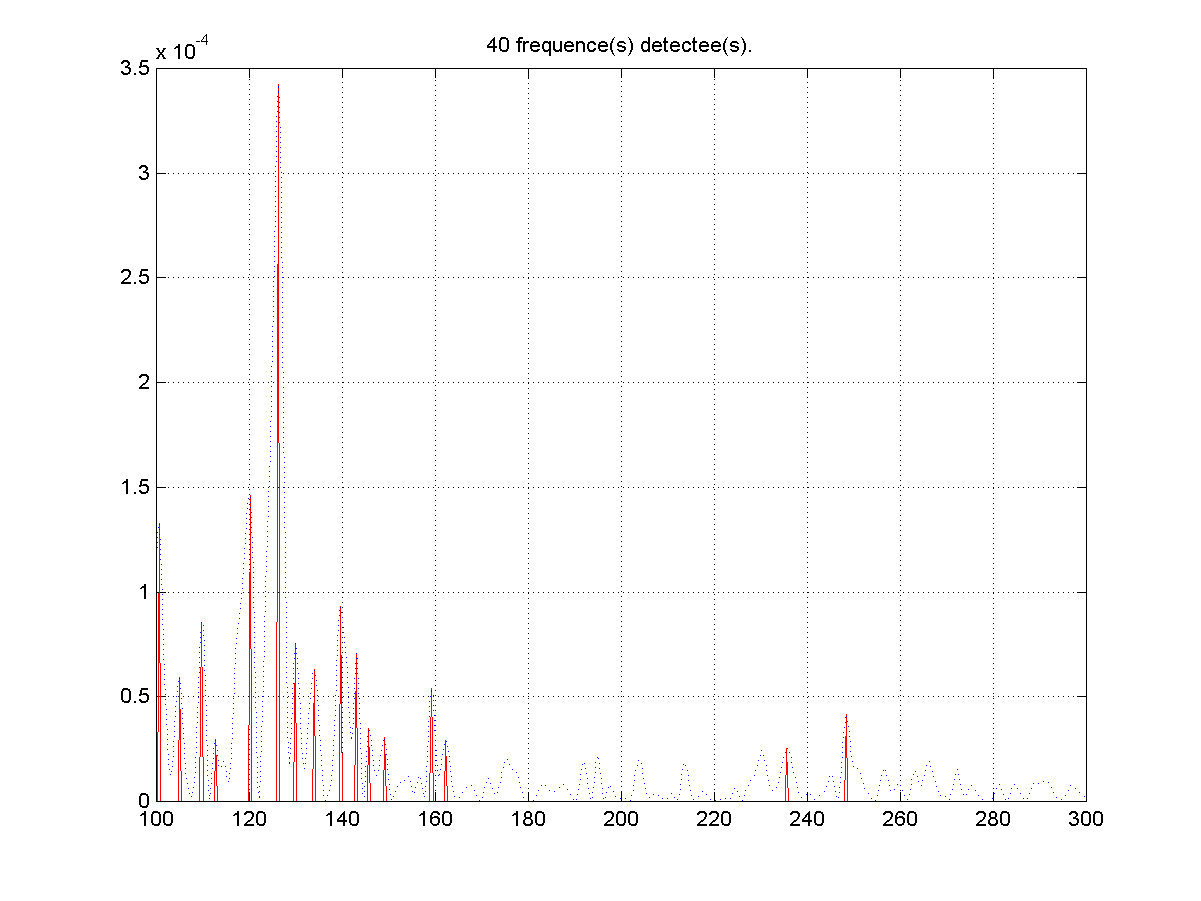
\includegraphics[width=12cm]{figures/tones.png}\\
      \caption{Affichage typique de la fonction {\tt get\_all\_tones} apr{\`e}s un zoom.}
      \label{figtones}
    \end{figure}
    \newpage


    \newpage
%    \bigskip
    \subsection{Get\_funds}
    \label{getfunds}
    La fonction {\tt array\_out = get\_funds( array\_in [, wid ] )}
    extrait les fr{\'e}quences fondamentales du tableau {\tt array\_in},
    c'est {\`a} dire les fr{\'e}quences qui ne sont pas un multiple d'une
    autre. Attention car {\tt array\_in} est bien un tableau
    de fr{\'e}quences seulement, ce n'est pas un tableau de couples
    fr{\'e}quences/amplitudes. Le tableau {\tt array\_out} contient
    donc toutes les fr{\'e}quences de {\tt array\_in} moins les
    fr{\'e}quences {\tt F(i)} qui v{\'e}rifient:

    $$\exists {\tt F0} \in {\tt array\_in},\exists {\tt n} \in \textbf{N}, \left|{\tt F(i)}-\frac{\tt
    F0}{\tt n}\right| \leq \frac{\tt wid}{2}$$

    La valeur par d{\'e}faut de {\tt wid} est de 4 Hz, l'exemple suivant
    montre bien l'influence de ce param{\`e}tre.

    \begin{verbatim}
        >> Frequ = [ 440, 885, 550, 1100, 1652 ];
        >> get_funds( Frequ )

        ans =

            440   550   885

        >> get_funds( Frequ, 10 )

        ans =

            440   550
    \end{verbatim}

    \newpage
%    \bigskip
    \subsection{Get\_harmonics et Get\_harm\_dir}
    \label{getharmonics}
    La fonction
    {\tt Harm = get\_harmonics( sig, fs, F0 [, wid, thr ])}
    cherche la suite harmonique dans le son {\tt
    sig} dont la fr{\'e}quence fondamentale est {\tt F0} ou {\tt
    F0}/2. Pour cela les fr{\'e}quences pures du son sont d{\'e}tect{\'e}es
    gr{\^a}ce {\`a} {\tt get\_all\_tones} avec le param{\`e}tre {\tt thr} (voir
    page \pageref{getalltones}). Alors, parmi les fr{\'e}quences
    d{\'e}tect{\'e}es, celles qui v{\'e}rifient :

    $$ {\tt F} \in \left[{\tt F0} - \frac{\tt wid}{2} , {\tt F0} + \frac{\tt
    wid}{2}\right] $$

    \noindent sont s{\'e}lectionn{\'e}es, o{\`u} {\tt wid} vaut 4 Hz par d{\'e}faut. Puis pour chacune de
    ces fr{\'e}quences {\tt F}, une s{\'e}quence de 5 portes de largeur {\tt wid}
    est g{\'e}n{\'e}r{\'e}e gr{\^a}ce {\`a} {\tt dirac\_sequence}, cette s{\'e}quence est
    alors multipli{\'e}e point {\`a} point par la \dsp des fr{\'e}quences
    pures du son (sortie {\tt peak} de la fonction
    {\tt get\_all\_tones} page \pageref{getalltones}). On regarde quel est le
    dernier {\'e}l{\'e}ment non nul, sa position (Hertz) est divis{\'e}e
    par son ordre, c'est alors une meilleure estimation de la
    fr{\'e}quence fondamentale. Ce cheminement est r{\'e}it{\'e}r{\'e} avec la
    nouvelle valeur de fondamentale, en g{\'e}n{\'e}rant une s{\'e}quence d'un
    nombre de portes {\'e}gal {\`a} 5 plus l'ordre trouv{\'e}. La boucle s'arr{\^e}te
    lorsque l'ordre trouv{\'e} {\`a} ce tour est le m{\^e}me que celui
    du tour pr{\'e}c{\'e}dent, ou bien lorsque la derni{\`e}re harmonique
    trouv{\'e}e est la plus grande possible.\\

    {\tt F0} peut {\^e}tre un tableau de plusieurs fr{\'e}quences, auquel
    cas le traitement d{\'e}crit pr{\'e}c{\'e}demment est appliqu{\'e} pour
    chacune d'elles. Mais attention au cas particulier o{\`u} {\tt F0}
    ne contient que 2 fr{\'e}quences, on recherche alors
    toutes les s{\'e}quences harmoniques dont la fondamentale est
    comprise entre {\tt F0(1)} et {\tt F0(2)}.Enfin, {\tt signal}
    peut {\^e}tre remplacer par le nom d'un
    fichier au format wave, alors l'argument {\tt fs} ne doit plus
    {\^e}tre pr{\'e}cis{\'e}.\\

    La sortie {\tt Harm} est un tableau de cellules, chacune
    d'elles contenant une s{\'e}quence harmonique, c'est {\`a} dire un
    tableau de couples fr{\'e}quences/amplitudes, les fr{\'e}quences
    {\'e}tant toutes multiples de la premi{\`e}re. Le tableau de cellules
    est class{\'e} par ordre croissant de fondamentale. Si {\tt Harm}
    n'est pas pr{\'e}cis{\'e}, la fonction sauvegarde les r{\'e}sultats dans
    un fichier texte portant le m{\^e}me nom que {\tt signal} si ce
    dernier est un nom de fichier wave, ou bien une cha{\^\i}ne de
    caract{\`e}re {\tt 'date,heure'} (sortie de now2str page
    \pageref{now2str}), le tout pr{\'e}c{\'e}d{\'e} de {\tt 'harmonics\_'}.\\

    La fonction {\tt get\_harm\_dir( dir [, F0, wid, thr ])}
    applique la fonction {\tt get\_harmonics} d{\'e}crite ci-dessus
    {\`a} tous les fichiers wave contenus dans le r{\'e}pertoire {\tt
    dir}.\\

    L'exemple suivant montre l'influence du param{\`e}tre {\tt wid}
    dans la longueur des s{\'e}quences d{\'e}tect{\'e}es, de plus on peut
    remarquer que dans ce cas la fr{\'e}quence de 130 Hz n'est pas la
    fondamentale.

    \label{exgetharmonics}
    \begin{verbatim}
    >> h = get_harmonics( '9_vh_100_2200ft', 130 );
    >> h{1}

    ans =

        65.2725  129.8721  194.8082
         0.0057    0.0174    0.0094

    >> h = get_harmonics( '9_vh_100_2200ft', 130, 10 ) ;
    >> h{1}

    ans =

       62.5809  128.0216  193.2941  256.3797  379.8592
        0.0144    0.0272    0.0091    0.0079    0.0092
    \end{verbatim}

    \newpage
%    \bigskip
    \subsection{Mean\_harmonics et analyse\_harm}
    \label{meanharmonics}
    Voici certainement la fonction de cette famille qui doit le
    plus servir.
    \begin{center}
    {\tt Harm = mean\_harmonics( fichiers [, F0, wid, thr ]) }
    \end{center}
    recherche dans tous les fichiers wave contenus dans la cellule
    {\tt fichiers} les suites harmoniques de fondamentales {\tt
    F0} et/ou {\tt F0/2}. {\tt get\_harmonics} s'applique sur
    chacun des fichiers avec les param{\`e}tres pass{\'e}s {\`a}
    {\tt mean\_harmonics}, puis les r{\'e}sultats sont rassembl{\'e}s dans un
    seul tableau de cellules en fusionnant les cellules repr{\'e}sentant les
    s{\'e}quences harmoniques de m{\^e}me fondamentale (voir {\tt fusion}
    page \pageref{fusion}), ou en ins{\'e}rant {\`a} la bonne place les
    nouvelles s{\'e}quences (voir {\tt insertion} page
    \pageref{insertion}).\\

    Il est possible de sp{\'e}cifier une cha{\^\i}ne de caract{\`e}res {\`a} la
    place de la cellule {\tt fichiers}, alors le traitement se
    fera sur tous les fichiers wave du r{\'e}pertoire courant dont le
    nom contient la cha{\^\i}ne pass{\'e}e en param{\`e}tre.\\

    L'utilisation de {\tt mean\_harmonics} est identique {\`a} celle
    de {\tt get\_harmonics} ( hormis pour le premier param{\`e}tre
    bien-s{\^u}r ). C'est {\`a} dire que l'on peut sp{\'e}cifier une fr{\'e}quence
    minimale et maximale pour les fondamentales des sequences {\`a}
    rechercher, ou encore une liste de fr{\'e}quences candidates. Le
    format de la sortie est identique, et si aucun argument de
    sortie n'est pr{\'e}cis{\'e}, les r{\'e}sultats sont enregistr{\'e}s dans un
    fichier texte dont le nom d{\'e}pend du premier argument d'entr{\'e}e.
    Si ce dernier est un tableau de noms de fichiers, alors le
    nom du fichier texte sera {\tt 'mean\_harm\_date,heure.txt'}, si {\`a}
    l'inverse le premier argument est la cha{\^\i}ne de caract{\`e}re {\tt
    'str'} le nom sera {\tt 'mean\_harm\_str.txt'}.\\

    La fonction {\tt analyse\_harm( dir [, F0, wid, thr, len, nf
    ])} pr{\'e}pare l'ensemble des sons au format wave du r{\'e}pertoire
    {\tt dir} gr{\^a}ce {\`a} la routine {\tt prepare\_dir} {\`a} laquelle on
    passe les param{\`e}tres {\tt len} et {\tt nf} (voir page
    \pageref{preparedir}). Puis {\tt mean\_harmonics} est
    appliqu{\'e}e sur chacun des sous-r{\'e}pertoires ainsi cr{\'e}{\'e}s. A noter
    que si les sons avaient deja {\'e}t{\'e} pr{\'e}par{\'e}s (lors d'un pr{\'e}c{\'e}dent
    appel, direct ou indirect, de {\tt prepare\_dir}), {\tt
    analyse\_harm} ne le refera pas.

    \newpage
    Le r{\'e}sultat de l'exemple suivant est {\`a} comparer avec celui de
    la fonction {\tt get\_harmonics} page
    \pageref{exgetharmonics}.

    \begin{verbatim}
    >> h = mean_harmonics( 'vh_100_2200ft', 130, 10 );
    >> h{1}

    ans =

      Columns 1 through 6

       66.6358  133.6402  199.2855  267.0829  331.4095  380.8685
        0.0151    0.0193    0.0092    0.0084    0.0083    0.0100

      Columns 7 through 8

      464.6461  776.2047
        0.0085    0.0107
   \end{verbatim}

%%%%%%%%%%%%%%%%%%%%%%%%%%%%%%%%%%%%%%%%%%%%%%%%%%%%%%%%%%%%%%%%%%%%


%%%%%%%%%%%%%%%%%%%%  FONCTIONS SIMPLIFICATION  %%%%%%%%%%%%%%%%%%%%
\newpage
\section{Fonctions pour la simplification des sons}
\label{secsimplification}

    %\newpage
    \bigskip
    \subsection{Clone\_wave}
    \label{clonewave}
    La fonction {\tt clone\_wave( wavfile [, adjust,  nb, wid, bw, tnmr ] )}
    permet de reproduire le fichier au format wave {\tt wavfile}
    en un fichier wave portant le m{\^e}me nom avec le pr{\'e}fixe {\tt
    SYNTH\_}. Le fichier {\tt wavfile} est d{\'e}coup{\'e} en plusieurs
    petits fichiers wave gr{\^a}ce {\`a} {\tt cut\_wavfile} (page
    \pageref{cutwavfile}), la fonction {\tt mean\_pertinents}
    est appel{\'e}e en lui passant les fichiers cr{\'e}{\'e}s, ainsi
    que les arguments {\tt nb}, {\tt wid}, {\tt bw} et {\tt tnmr}
    (voir page \pageref{meanpertinents} pour plus de d{\'e}tails).
    Alors avec les caract{\'e}ristiques ainsi extraites, un son de m{\^e}me
    longueur et de m{\^e}me niveau que l'original peut {\^e}tre synth{\'e}tis{\'e}
    gr{\^a}ce {\`a} la fonction {\tt synthetize} (page
    \pageref{synthetize}) {\`a} qui on passe {\tt adjust}. Cela permet de v{\'e}rifier que la
    mod{\'e}lisation est bien adapt{\'e}e aux types de sons trait{\'e}s, et
    {\'e}ventuellement d'affiner les param{\`e}tres du model.\\

    Il est {\'e}galement possible de se servir de cette fonction
    sous la forme:
    \begin{center}
    {\tt clone\_wave( wavcell [, nb, wid, bw, tnmr ] )},
    \end{center}
    o{\`u} {\tt wavcell} est le tableau des noms de fichier wave {\`a}
    traiter avec {\tt clone\_wave}.


    \newpage
    %\bigskip
    \subsection{Decimation}
    \label{decimation}
    La fonction
    \begin{center}
    {\tt [ppsd, rpsd] = decimation( odsp, tpsd, FS [, nb, bw, TNMR ] )}
    \end{center}
    permet de simplifier un son complexe stationnaire en
    ne gardant que {\tt nb} composantes tonales (20 par d{\'e}faut) de
    la \dsp des fr{\'e}quences pures {\tt tpsd} produite par {\tt get\_all\_tones}
    (page \pageref{getalltones}). La \dsp d'origine {\tt opsd} est
    {\'e}galement n{\'e}cessaire pour deux raisons. Premi{\`e}rement pour
    v{\'e}rifier que chacune des raies spectrales n'est pas masqu{\'e}e
    par le bruit qui l'entoure. En second lieu, le mod{\`e}le de
    synth{\`e}se choisi remplace tout ce qui n'est pas retenu de la \dsp
    originale en bande de bruit d'{\'e}nergie moyenne {\'e}quivalente.\\

    Voici comment est effectu{\'e}e la s{\'e}lection. Pour chacune des raies
    spectrales, une fen{\^e}tre de largeur {\tt bw} bark (1
    par d{\'e}faut) centr{\'e}e g{\'e}ometriquement sur la raie est d{\'e}finie gr{\^a}ce {\`a} la
    fonction {\tt critical\_band} (page \pageref{criticalband}),
    on v{\'e}rifie alors que la raie concern{\'e}e d{\'e}passe de plus de
    {\tt TNMR} dB (5 dB par d{\'e}faut) le niveau d'{\'e}nergie moyen
    contenu dans cette bande. Si ce n'est pas le cas, le ton
    est masqu{\'e} par le bruit environnant, sinon il faut v{\'e}rifier
    que la raie consid{\'e}r{\'e}e est la plus grande dans cette m{\^e}me bande,
    alors seulement elle est consid{\'e}r{\'e}e comme {\'e}tant une
    composante tonale pertinente.
    Cette m{\'e}thode est une approximation du masquage tonale, en
    effet le v{\'e}ritable ph{\'e}nom{\`e}ne de masquage fait intervenir des
    pentes autour de la fr{\'e}quence consid{\'e}r{\'e}e, mais cela suffit
    pour notre besoin. Il suffit ensuite de garder les {\tt nb}
    fr{\'e}quences dont les amplitudes (pond{\'e}r{\'e}es par le seuil
    d'audition absolue) sont les plus importantes.\\

    \newpage
    Sont r{\'e}cup{\'e}r{\'e}s {\tt ppsd} une \dsp constitu{\'e}e uniquement des {\tt nb}
    tons jug{\'e}s les plus pertinents, et {\tt rpsd} qui contient
    la \dsp originale {\`a} laquelle sont retir{\'e}es les susdites fr{\'e}quences pertinentes.
    Si {\tt nb} est nul, on garde toutes les fr{\'e}quences pures qui ne sont pas masqu{\'e}es
    par le bruit et qui sont les plus importantes de leur bande critique.

    \medskip
    \begin{figure}[h]
      \centering
      \begin{verbatim}
      >> [f, tdsp, dsp] = get_all_tones('9_vh_100_2200ft');
      >> fs=44100;
      >> [ddsp, rdsp] = decimation(dsp,tdsp,44100);
      >> incr = fs/(2*length(dsp)); F=0:incr:fs/2-incr;
      >> plot(F,tdsp,F,ddsp)
      \end{verbatim}
      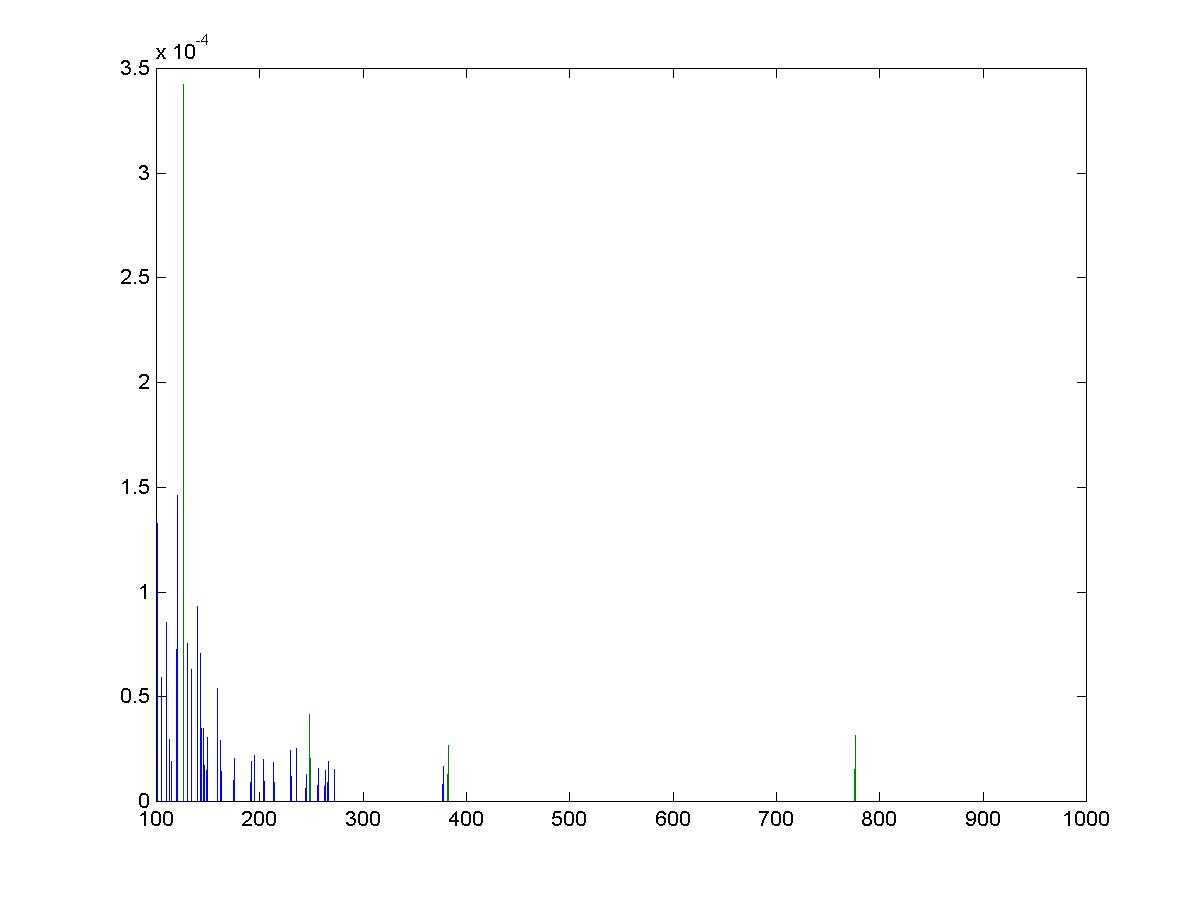
\includegraphics[width=12cm]{figures/decimation.png}\\
      \caption{Comparaison entre les tons jug{\'e}s pertinents (vert) et l'ensemble des tons pr{\'e}sents (bleu).}
      \label{figdecimation}
    \end{figure}


    \newpage
    %\bigskip
    \subsection{Get\_noise\_band}
    \label{getnoiseband}
    La fonction {\tt noises = get\_noise\_band( PSD, fs , len [, nbw ])} s{\'e}pare
    la \dsp {\tt PSD} en bandes contig{\"u}es de {\tt nbw} bark de
    large (1 bark par d{\'e}faut), et sur chacune d'elles moyenne
    l'{\'e}nergie. Ainsi {\tt noises} est un tableau de $\frac{25}{\tt nbw}$
    niveaux de bruit. {\tt len} est le nombre d'{\'e}chantillons du signal original,
    avant zero-padding, cette longueur est n{\'e}cessaire pour calculer le niveau d'{\'e}nergie.
    Typiquement {\tt PSD} est le deuxi{\`e}me argument
    de sortie de {\tt decimation} (page \pageref{decimation}).
    Le tableau ne regroupe que les niveaux de bandes de bruit,
    soit la racine carr{\'e}e de la variance de la bande consid{\'e}r{\'e}e,
    il suffira ainsi de multiplier simplement cette valeur par
    la \dsp dans la bande consid{\'e}r{\'e}e. A noter que si {\tt nbw} est
    {\'e}gal {\`a} 0, la fonction est court-circuit{\'e}e et {\tt noises} a
    pour valeur {\tt PSD}. Mais attention, ceci ne peut {\^e}tre
    utilis{\'e} directement avec {\tt synthetize}.\\


    \newpage
    %\bigskip
    \subsection{Get\_pertinents et get\_pert\_dir}
    \label{getpertinents}
    La fonction
    \begin{center}
    {\tt [tone, noise, cbt] = get\_pertinents( s, fs [, n, bw, r, win ])}
    \end{center}
    retourne les param{\`e}tres jug{\'e}s pertinents {\`a} l'oreille du signal
    {\tt s} {\'e}chantillonn{\'e} {\`a} la fr{\'e}quence {\tt fs}. Il est
    {\'e}galement possible de pr{\'e}ciser le nombre {\tt n} de fr{\'e}quences {\`a}
    garder (par d{\'e}faut 20), si on veut toutes les garder il suffit de
    mettre {\tt n} {\`a} 0. Les largeurs d'analyse en bark sont
    pass{\'e}es par le param{\`e}tre {\tt bw}, ainsi {\tt bw(1)} est la
    largeur de la fen{\^e}tre de masquage fr{\'e}quentiel, et {\tt bw(2)}
    celle des bandes de bruit (par d{\'e}faut {\tt bw = [ 0.5, 1 ]}),
    {\`a} noter que si {\tt bw} est un scalaire, ce sera {\tt bw(1)}
    et {\tt bw(2)} sera mis {\`a} sa valeur par d{\'e}faut de 1 bark.
    {\tt r} est le rapport en dB en dessous duquel une
    fr{\'e}quence pure est masqu{\'e}e par le bruit avoisinant (c'est {\`a}
    dire l'{\'e}nergie contenue dans la bande de {\tt bw(1)} bark de
    large centr{\'e}e sur la fr{\'e}quence en question), par d{\'e}faut {\tt
    r} est de 5 dB. Enfin {\tt win} permet de sp{\'e}cifier le type
    de fen{\^e}tre temporelle {\`a} utiliser avant de calculer la \dsp (par
    d{\'e}faut une fen{\^e}tre de Hanning est utilis{\'e}e).\\

    La d{\'e}marche est la suivante, on recherche toutes les fr{\'e}quences
    pures pr{\'e}sentes dans le signal avec la fonction {\tt get\_all\_tones}
    (page \pageref{getalltones}) {\`a} laquelle on passe le param{\`e}tre
    {\tt win}, les {\tt nb} fr{\'e}quences jug{\'e}es les plus importantes sont
    s{\'e}lectionn{\'e}es gr{\^a}ce {\`a} {\tt decimation} (page \pageref{decimation})
    qui prend en param{\`e}tres {\tt nb}, {\tt bw(1)} et {\tt r}.
    Enfin, la \dsp diminu{\'e}e des fr{\'e}quences s{\'e}lectionn{\'e}es est
    partag{\'e}e en bande de largeur {\tt bw(2)} bark, et sur chacune d'elles
    le niveau d'{\'e}nergie est moyenn{\'e}.\\

    On r{\'e}cup{\`e}re donc un tableau {\tt tone} de couple
    fr{\'e}quences/amplitudes, un tableau de niveaux de bandes de
    bruit {\tt noise}. Le dernier argument de sortie est
    {\'e}galement un tableau de couples fr{\'e}quences/amplitudes, mais
    les fr{\'e}quences gard{\'e}es sont les plus pertinentes pour chacune
    des bandes de bruit. En d'autres termes, il y aura autant de
    fr{\'e}quences pures s{\'e}lectionn{\'e}es que de bandes de bruit.\\

    La fonction {\tt get\_pert\_dir( dir [, n, bw, r, win ] )}
    applique {\tt get\_pertinents} {\`a} tous les fichiers wave
    contenus dans le r{\'e}pertoire {\tt dir}.


    \newpage
    %\bigskip
    \subsection{Get\_pert\_harm}
    \label{getpertharm}
    La fonction
    \begin{center}
    {\tt [harm, tone, noise] = get\_pert\_harm( file [, n, w, bw ])}
    \end{center}
    recherche les sequences harmoniques dans le fichier wave
    {\tt file} dont le fondamental (et/ou le premier harmonique)
    est une fr{\'e}quence jug{\'e}e pertinente au sens psychoacoustique.
    Pour cela, la fonction {\tt get\_pertinents} est appel{\'e}e avec
    les arguments {\tt n} et {\tt bw} (voir page \pageref{getpertinents}),
    les fr{\'e}quences r{\'e}cup{\'e}r{\'e}es sont transmises {\`a} {\tt get\_funds}
    avec le param{\`e}tre {\tt w} (voir page \pageref{getfunds}),
    {\'e}liminant ainsi toutes fr{\'e}quences multiples, celles qui restent
    sont alors envoy{\'e}es {\`a} la fonction {\tt get\_harmonics} avec le
    param{\`e}tre {\tt w} (voir page \pageref{getharmonics}).\\

    La fonction retourne un tableau de cellules contenant les s{\'e}quences
    harmoniques trouv{\'e}es ({\tt harm}), le tableau des couples
    fr{\'e}quences/amplitudes jug{\'e}s pertinents {\tt tone} et le tableau des niveaux
    de bruits ({\tt noise}). Si aucun argument de sortie n'est
    pr{\'e}cis{\'e}, les r{\'e}sultats sont enregistr{\'e}s dans un fichier texte
    portant le m{\^e}me nom que le fichier wave {\tt file} avec le
    pr{\'e}fixe {\tt 'pert\_harm\_'}.


    \newpage
    %\bigskip
    \subsection{Mean\_pertinents et analyse\_pert}
    \label{meanpertinents}
    La fonction
    \begin{center}
    {\tt [tones, noises, cbt] = mean\_pertinents( files [, n, w, bw, r ])}
    \end{center}
    permet d'effectuer la recherche des composantes pertinentes dans
    un ensemble de fichiers wave repr{\'e}sentant le m{\^e}me son,
    l'argument {\tt file} est alors une cellule contenant les noms
    des fichiers {\`a} traiter.\\

    On proc{\`e}de de la mani{\`e}re suivante: un tableau
    {\tt hits} de triplet (fr{\'e}quences, niveaux cumul{\'e}s, hit)
    est cr{\'e}{\'e} {\`a} partir des sorties de la fonction {\tt get\_pertinents}
    appliqu{\'e}e {\`a} chacun des fichiers de {\tt files}, ainsi chaque
    fois qu'une fr{\'e}quence deja pr{\'e}sente dans {\tt hits}
    est {\`a} nouveau jug{\'e}e comme pertinente, son amplitude est
    ajout{\'e}e
    au niveau cumul{\'e} et le compteur hit est incr{\'e}ment{\'e}. Puis,
    lorsque l'ensemble des fichiers a {\'e}t{\'e} trait{\'e}, les {\tt n}
    fr{\'e}quences dont les niveaux cumul{\'e}s (pond{\'e}r{\'e}s par le seuil
    d'audition) sont les plus importants, sont s{\'e}lectionn{\'e}es,
    l'int{\'e}r{\^e}t de ce type de selection est qu'elle tient compte {\`a}
    la fois du niveau et du nombre d'apparitions des fr{\'e}quences.
    Ainsi une fr{\'e}quence qui appara{\^\i}t tr{\`e}s souvent,
    m{\^e}me avec un niveau moyen, sera privil{\'e}gi{\'e}e face {\`a} une fr{\'e}quence qui ne serait
    pr{\'e}sente que dans un seul fichier, m{\^e}me avec un niveau
    important. On s'affranchit donc des accidents de prise de
    son.\\

    Sont r{\'e}cup{\'e}r{\'e}s un tableau {\tt tones} de couple
    fr{\'e}quences/amplitudes (les amplitudes {\'e}tant simplement
    r{\'e}cup{\'e}r{\'e}es en divisant le niveau cumul{\'e} par le nombre
    de hit), un tableau de niveaux moyens de bandes de bruit
    {\tt noises}. Le dernier argument de sortie est {\'e}galement
    un tableau de couples fr{\'e}quences/amplitudes ne contenant que
    les fr{\'e}quences les plus pertinentes pour chacune
    des bandes de bruit. Si aucun argument de sortie n'est pr{\'e}cis{\'e},
    les r{\'e}sultats sont enregistr{\'e}s dans un fichier texte.\\

    La fonction {\tt analyse\_pert( dir [, n, w, bw, r, len, nf
    ])} pr{\'e}pare l'ensemble des sons au format wave du r{\'e}pertoire
    {\tt dir} gr{\^a}ce {\`a} la routine {\tt prepare\_dir} {\`a} laquelle on
    passe les param{\`e}tres {\tt len} et {\tt nf} (voir page
    \pageref{preparedir}). Puis {\tt mean\_pertinents} est
    appliqu{\'e}e sur chacun des sous-r{\'e}pertoires ainsi cr{\'e}{\'e}. A noter
    que si les sons avaient d{\'e}j{\`a} {\'e}t{\'e} pr{\'e}par{\'e}s (lors d'un pr{\'e}c{\'e}dent
    appel, direct ou indirect, de {\tt prepare\_dir}), {\tt
    analyse\_pert} ne le refera pas.


    \newpage
    %\bigskip
    \subsection{Mean\_pert\_harm et analyse\_pert\_harm}
    \label{meanpertharm}
    La fonction
    \begin{center}
    {\tt [Harm, tone, noise] = mean\_pert\_harm( files [, n, w, bw, r])}
    \end{center}
    effectue le m{\^e}me type de traitement que {\tt
    get\_pertinent\_harms} (page \pageref{getpertharm}) mais
    sur un ensemble de fichiers wave repr{\'e}sentant le m{\^e}me son.
    Pour ce faire, on commence par appliquer {\tt mean\_pertinents}
    (voir page \pageref{meanpertinents}), puis sont s{\'e}lectionn{\'e}es
    parmi les fr{\'e}quences jug{\'e}es pertinentes les candidates {\`a} {\^e}tre
    fondamentales gr{\^a}ce {\`a} {\tt get\_funds} (voir page
    \pageref{getfunds}), enfin les s{\'e}quences harmoniques
    sont recherch{\'e}es avec {\tt mean\_harmonics} (voir page
    \pageref{meanharmonics}).\\

    A l'instar de toutes les fonctions pr{\'e}fix{\'e}es par {\tt mean\_},
    l'argument {\tt files} peut {\^e}tre un tableau des noms des
    fichiers {\`a} analyser, ou une cha{\^\i}ne de caract{\`e}res, dans ce
    cas la fonction appliquera son traitement sur tous les
    fichiers wave du r{\'e}pertoire courant dont le nom contient la
    cha{\^\i}ne.\\

    La sortie {\tt Harm} est un tableau de s{\'e}quences
    harmoniques, {\tt tones} est le tableau de couples
    fr{\'e}quences/amplitudes jug{\'e}s pertinents, et enfin {\tt noises}
    et le niveau de chaque bande de bruits. Si il n'y a aucun
    argument de sortie, les r{\'e}sultats sont sauvegard{\'e}s dans un
    fichier texte dont le nom est {\tt 'mean\_pert\_harm\_str.txt'}
    si le premier argument est une cha{\^\i}ne de caract{\`e}res,
    {\tt 'mean\_pert\_harm\_date,heure.txt'} si le premier argument
    est un tableau de noms de fichier.\\

    La fonction {\tt analyse\_pert\_harm( dir [, n, w, bw, r, len, nf
    ])} pr{\'e}pare l'ensemble des sons au format wave du r{\'e}pertoire
    {\tt dir} gr{\^a}ce {\`a} la routine {\tt prepare\_dir} {\`a} laquelle on
    passe les param{\`e}tres {\tt len} et {\tt nf} (voir page
    \pageref{preparedir}). Puis {\tt mean\_pertinent\_harms} est
    appliqu{\'e}e sur chacun des sous-r{\'e}pertoires ainsi cr{\'e}{\'e}s. A noter
    que si les sons avaient d{\'e}j{\`a} {\'e}t{\'e} pr{\'e}par{\'e}s (lors d'un pr{\'e}c{\'e}dent
    appel, direct ou indirect, de {\tt prepare\_dir}), {\tt
    analyse\_pert\_harm} ne le refera pas.


    \newpage
    %\bigskip
    \subsection{Synthetize}
    \label{synthetize}
    La fonction {\tt signal = synthetize( tones [, noises, adjust, fs, s, nf])}
    est le g{\'e}n{\'e}rateur de signal de cette boite {\`a} outils.
    L'argument d'entr{\'e}e {\tt tones} est un tableau 2 lignes, n
    colonnes repr{\'e}sentant les couples fr{\'e}quences/amplitudes des
    sinus que l'on veut additionner. {\tt noises} est un vecteur
    de niveau par bandes de bruit, ainsi le spectre audible est
    s{\'e}par{\'e} en autant de bandes de largeur fixe (dans l'{\'e}chelle des
    barks) qu'il a de case {\`a} {\tt noises}, la \dsp du signal de
    sortie aura alors pour chacune de ces bandes la valeur
    correspondante du tableau {\tt noises} multipli{\'e}e par {\tt adjust}
    (1 par d{\'e}faut), en effet il est apparu que pour des sons tr{\`e}s riches
    en fr{\'e}quences pures, le son synth{\'e}tis{\'e} directement avec les niveaux de bruit
    calcul{\'e}s semble trop bruit{\'e}, dans ce cas un {\tt adjust} inf{\'e}rieur {\`a} 1 permet
    de corriger cet effet. Si on veut g{\'e}n{\'e}rer un signal
    uniquement constitu{\'e} de bruit, il suffit de mettre [] {\`a} la place de
    {\tt tones}.Par d{\'e}faut, {\tt
    noises} est nul, ce qui {\'e}quivaut {\`a} un signal sans bruit. Il
    est {\'e}galement possible de pr{\'e}ciser la fr{\'e}quence d'{\'e}chantillonnage du
    signal gr{\^a}ce {\`a} {\tt fs} (44,1kHz par d{\'e}faut), la dur{\'e}e en
    seconde du signal avec {\tt s} ($\frac{32768}{\tt fs}$ par
    d{\'e}faut, soit un signal de 32768 {\'e}chantillons). Enfin {\tt nf}
    permet la normalisation en amplitude du signal ({\tt nf = 1}),
    ce qui peut {\^e}tre n{\'e}cessaire dans le cas d'un signal g{\'e}n{\'e}r{\'e}
    trop faible (inaudible), ou {\`a} l'inverse trop fort
    (saturation). Par d{\'e}faut la normalisation n'est pas active
    ({\tt nf = 0}).\\

    Une version avec deux arguments de sortie {\tt
    tonal} et {\tt noisy} est disponible, dans ce cas
    les partie tonale (uniquement constitu{\'e}e de sinuso{\"\i}des) et la
    bruit{\'e}e (uniquement constitu{\'e}e de bandes de bruit de
    largeur constante dans l'{\'e}chelle des barks) sont s{\'e}par{\'e}es. Il est alors
    possible de reconstituer le signal final en additionnant ces
    deux vecteurs. Si trois arguments de sortie sont cit{\'e}s, ce
    seront respectivement le signal total, la fr{\'e}quence
    d'{\'e}chantillonnage et 16 repr{\'e}sentant le nombre de bits de
    quantification. Ceci permet d'avoir, si besoin est, une sortie
    homog{\`e}ne {\`a} celle de la fonction {\tt wavread}. Enfin,
    l'absence de param{\`e}tre de sortie implique que le son
    synth{\'e}tis{\'e} sera enregistr{\'e} dans le r{\'e}pertoire courant au
    format wave, son nom sera {\tt 'SYNTH\_date,heure.wave'}.

%%%%%%%%%%%%%%%%%%%%%%%%%%%%%%%%%%%%%%%%%%%%%%%%%%%%%%%%%%%%%%%%%%%%


%%%%%%%%%%%%%%%%%%%%%%%  FONCTIONS ANNEXES  %%%%%%%%%%%%%%%%%%%%%%%%
\newpage
\section{Fonctions annexes}
\label{secannexes}


    %\newpage
    \bigskip
    \subsection{Cell2file}
    \label{cell2file}
    La fonction {\tt cell2file( carray, file [, nb\_min])}
    enregistre de la mani{\`e}re la plus lisible le tableau de
    cellules {\tt carray} dans le fichier {\tt file}. {\tt carray}
    est typiquement la sortie de {\tt get\_harmonics} ou {\tt mean\_harmonics}...
    Si {\tt file} existe d{\'e}j{\`a}, la sauvegarde se fait {\`a} la suite
    du fichier.\\

    Le param{\`e}tre {\tt nb\_min} permet de pr{\'e}ciser la longueur
    minimale des cellules {\`a} sauvegarder, par d{\'e}faut {\`a} 1.\\

    Il existe aussi la forme
    \begin{center}
    {\tt cell2file( carray, file , header [, nb\_min])}
    \end{center}
    \noindent il est possible de sp{\'e}cifier une ent{\^e}te {\tt header} qui sera
    {\'e}crite juste avant les donn{\'e}s proprement dites.\\

    Enfin, le param{\`e}tre {\tt file} peut {\^e}tre remplac{\'e} par un
    identifiant de fichier, c'est {\`a} dire la valeur de retour de la
    fonction \matlab {\tt fopen}. Dans ce cas, le fichier ne sera
    pas ferm{\'e} {\`a} l'int{\'e}rieur de {\tt cell2file}. C'est {\`a}
    l'utilisateur de faire appel {\`a} la fonction \matlab {\tt
    fclose}.


    \newpage
    %\bigskip
    \subsection{Cell\_fusion}
    \label{cellfusion}
    La fonction {\tt cout = cell\_fusion( cin1, cin2 [, wid ] )}
    permet de fusionner deux tableaux de cellules {\tt cin1} et
    {\tt cin2} pour n'en faire qu'un seul {\tt cout}. Ainsi les cellules
    repr{\'e}sentant les m{\^e}mes s{\'e}quences harmoniques seront fusionn{\'e}es
    gr{\^a}ce {\`a} {\tt fusion} (page \pageref{fusion}.
    Sont consid{\'e}r{\'e}e comme repr{\'e}sentant la
    m{\^e}me s{\'e}quence harmonique deux cellules dont les fr{\'e}quences fondamentales
    respectives {\tt F1} et {\tt F2} v{\'e}rifient l'une des relations
    suivantes:

    $$ \left|{\tt F0}-{\tt F1}\right| \leq \frac{\tt wid}{2} $$
    \begin{center} ou \end{center}
    $$ \left|\frac{\tt F0}{2}-{\tt F1}\right| \leq \frac{\tt wid}{2} $$
    \begin{center} ou encore \end{center}
    $$ \left|{\tt F0}-\frac{\tt F1}{2}\right| \leq \frac{\tt wid}{2} $$

    \bigskip
    La valeur de {\tt wid} est de 4 Hz par d{\'e}faut. Attention tout
    de m{\^e}me que les tableaux de cellules {\`a} fusionner soient class{\'e}s
    par ordre croissant de fondamentaux pour que l'algorithme
    marche, on pourra donc utiliser {\tt cell\_sort} (page \pageref{cellsort}).

    \begin{verbatim}
        >> c1{1} = [ 440*(1:1:4)', ones(4,1) ]';
        >> c1{2} = [ 550*(1:1:3)', ones(3,1) ]';
        >> c2{1} = [ 880*(1:1:4)', 2*ones(5,1) ]';
        >> c2{2} = [ 555*(1:2:4)' 2*ones(4,1) ]';
        >> c3 = cell_fusion( c1, c2 )

        c3 =

            [2x6 double]    [2x3 double]    [2x4 double]

        >> c3{1}, c3{2}, c3{3}

        ans =

          1.0e+003 *

            0.4400    0.8800    1.3200    1.7600    2.6400    3.5200
            0.0010    0.0015    0.0010    0.0015    0.0020    0.0020


        ans =

             550        1100        1650
               1           1           1


        ans =

             555        1665        2775        3885
               2           2           2           2


        >> c3 = cell_fusion( c1, c2, 10 )

        c3 =

            [2x7 double]    [2x5 double]

        >> c3{1}, c3{2}

        ans =

          1.0e+003 *

            0.4400    0.8800    1.3200    1.7600    2.6400    3.5200
            0.0010    0.0015    0.0010    0.0015    0.0020    0.0020


        ans =

          1.0e+003 *

            0.5525    1.1000    1.6575    2.7625    3.8850
            0.0015    0.0010    0.0015    0.0015    0.0020
    \end{verbatim}


    %\newpage
    \bigskip
    \subsection{Cell\_sort}
    \label{cellsort}
    La fonction {\tt cout = cell\_sort( cin )} permet de classer
    le tableau de cellules {\tt cin} dans l'ordre croissant de ses
    fondamentaux.

    \begin{verbatim}
        >> c = cell(1,3);
        >> c{1} = [ 680*(1:5)', ones(5,1)]';
        >> c{2} = [ 550*(1:3)', ones(3,1)]';
        >> c{3} = [ 1000*(1:6)', ones(6,1)]';
        >> c = cell_sort( c );
        >> c{1}(1,1), c{2}(1,1), c{3}(1,1)

        ans =

           550


        ans =

           680


        ans =

          1000
        \end{verbatim}


    %\newpage
    \bigskip
    \subsection{Cut\_wavfile}
    \label{cutwavfile}
    La function {\tt cut\_wavfile( wavfile [, dirout, len, nf ] )}
    d{\'e}coupe le fichier wave {\tt wavfile} en plusieurs fichiers au
    format wave de longueur {\tt len} (32768 {\'e}chantillons par
    d{\'e}faut), les enregistre dans le r{\'e}pertoire {\tt dirout}
    (r{\'e}pertoire courant par d{\'e}faut). Le format des noms des
    fichiers ainsi cr{\'e}{\'e}s est le suivant : 'X\_nomdorigine.wav' si
    le fichier d'origine est mono, 'voieY\_X\_nomdorigine.wav' si le
    fichier d'origine est st{\'e}r{\'e}o. Le dernier param{\`e}tre {\tt nf}
    permet de sp{\'e}cifier si les fichiers ainsi cr{\'e}{\'e}s seront
    normalis{\'e}s en amplitude ({\tt nf = 1}) ou pas ({\tt nf = 0}
    valeur par d{\'e}faut).


    %\newpage
    \bigskip
    \subsection{Fusion}
    \label{fusion}
    La fonction {\tt out = fusion( in1, in2 )} permet, {\`a}
    partir des deux tableaux repr{\'e}sentant la m{\^e}me s{\'e}quence harmonique,
    de n'en faire qu'un. Deux fr{\'e}quences {\tt F1} et {\tt F2} seront alors consid{\'e}r{\'e}es
    comme {\'e}gales si elles correspondent au m{\^e}me ordre
    d'harmonique, c'est {\`a} dire si elles v{\'e}rifient:

    $$ round \( \frac{\tt F1 - F2}{\tt F0} \) = 0 $$

    \noindent o{\`u} {\tt F0} est la fr{\'e}quence fondamentale des deux
    s{\'e}quences. Le tableau {\tt out} contient donc toutes les
    fr{\'e}quences de {\tt in1} et {\tt in2}, avec l'amplitude
    et la fr{\'e}quence moyenne l{\`a} o{\`u} ces derni{\`e}res co{\"\i}ncident. Voici
    un exemple de fusion de deux s{\'e}quences harmoniques:

    \begin{verbatim}
    >> a = [ 440*(1:5)', ones(5,1) ]';
    >> b = [ 480*(1:6)', 2*ones(6,1) ]';
    >> fusion( a, b )

    ans =

      1.0e+003 *

        0.4600    0.9200    1.3800    1.8400    2.3000    2.8800
        0.0015    0.0015    0.0015    0.0015    0.0015    0.0020
    \end{verbatim}


    %\newpage
    \bigskip
    \subsection{Get\_all\_dir}
    \label{getalldir}
    La fonction {\tt subdir = get\_all\_dir( [ dir ] ) } recherche
    tous les sous-r{\'e}pertoires du r{\'e}pertoire {\tt dir} (r{\'e}pertoire
    courant par d{\'e}faut), puis cr{\'e}e un tableau {\tt subdir}
    contenant les noms des sous-r{\'e}pertoires trouv{\'e}s. On peut voir
    un exemple d'utilisation de cette fonction:
    \begin{verbatim}
        >> cd PREPARED
        >> subdir = get_all_dir;
        >> subdir( 2 )

        ans =

        'vh_100_2200ft'
    \end{verbatim}


    %\newpage
    \bigskip
    \subsection{Get\_all\_files}
    \label{getallfiles}
    La fonction {\tt noms = get\_all\_files( str )} retourne un
    tableau contenant les noms des fichiers wave dont le nom
    contient la cha{\^\i}ne de caract{\`e}res {\tt str}. Voici un exemple
    d'utilisation de cette fonction:
    \begin{verbatim}
        >> files = get_all_files( 'vh_100' );
        >> files(3)

        ans =

            '12_vh_100_2200ft.wav'
    \end{verbatim}


    %\newpage
    \bigskip
    \subsection{Insertion}
    \label{insertion}
    {\tt Cout = insertion( array, Cin, index )} permet d'ins{\'e}rer
    le tableau de couples fr{\'e}quences/amplitudes {\tt array} dans
    le tableau de cellules {\tt Cin}, {\`a} la cellule {\tt index}.
    L'exemple suivant illustre les possibilit{\'e}s de cette fonction:

    \begin{verbatim}
        >> c = cell(1,2);
        >> c{1} = 'debut'; c{2} = 'fin';
        >> c

        c =

        'debut'    'fin'

        >> c = insertion('au milieu',c,2)

        c =

        'debut'    'au milieu'    'fin'

        >> c = insertion('apres',c,4)

        c =

        'debut'    'au milieu'    'fin'    'apres'
    \end{verbatim}


    %\newpage
    \bigskip
    \subsection{Noises2file}
    \label{noises2file}
    La fonction {\tt noises2file( noises, file [, header ] )}
    permet d'enregistrer le tableau de niveaux de bruit {\tt
    noises} dans le fichier nomm{\'e} {\tt file}. On peut ajouter un
    texte {\`a} {\'e}crire avant les donn{\'e}es gr{\^a}ce {\`a} {\tt header}.
    L'argument {\tt file} peut {\^e}tre remplac{\'e} par un
    identifiant de fichier, c'est {\`a} dire la valeur de retour de la
    fonction \matlab {\tt fopen}. Dans ce cas, le fichier ne sera
    pas ferm{\'e} {\`a} l'int{\'e}rieur de {\tt cell2file}. C'est {\`a}
    l'utilisateur de faire appel {\`a} la fonction \matlab {\tt
    fclose}.


    %\newpage
    \bigskip
    \subsection{Now2str}
    \label{now2str}
    La fonction {\tt str = now2str([ f ])}
    convertit le flottant {\tt f}, sortie de la fonction \matlab
    {\tt now}, en une cha{\^\i}ne de caract{\`e}res {\tt str} representant la date
    et l'heure. Si {\tt f} n'est pas pr{\'e}cis{\'e}, l'appel de {\tt now}
    se fait {\`a} l'int{\'e}rieur de la fonction. L'exemple suivant l'illustre.

    \begin{verbatim}
        >> n = now;
        >> now2str( n )

        ans =

        18-Jul-2002,17h59mn44s

        >> now2str

        ans =

        18-Jul-2002,17h59mn58s
    \end{verbatim}


    \newpage
    %\bigskip
    \subsection{Prepare\_dir}
    \label{preparedir}
    La fonction {\tt prepare\_dir([ dir, len, nf ])} pr{\'e}pare de
    mani{\`e}re automatique les fichiers wave contenus dans le
    r{\'e}pertoire {\tt dir} (le r{\'e}pertoire courant si non pr{\'e}cis{\'e})
    en vue de leur traitement ult{\'e}rieur. Un
    sous-r{\'e}pertoire nomm{\'e} {\tt 'PREPARED'} est cr{\'e}{\'e}, puis {\`a}
    l'int{\'e}rieur de ce dernier, autant de sous-r{\'e}pertoires qu'il n'y
    a de fichiers wave. Chacun de ces sous-r{\'e}pertoires portant le
    nom d'un fichier wave ({\`a} l'extension pr{\`e}s bien s{\^u}r). Puis la
    fonction {\tt cut\_wavfile} entre en sc{\`e}ne, avec les
    param{\`e}tres {\tt dir}, {\tt len} et {\tt nf}, les r{\'e}sultats
    {\'e}tant rang{\'e}s dans le sous-r{\'e}pertoire appropri{\'e}. Les valeurs par
    d{\'e}faut sont: {\tt len = 32768} et {\tt nf = 0} c'est {\`a} dire
    que la normalisation est d{\'e}sactiv{\'e}e. Voici un
    exemple de l'utilisation de cette fonction:

    \begin{verbatim}
        >> dir

        .       ..      vh_80_2200ft.wav    vh_100_2200ft.wav

        >> prepare_dir
        >> dir

        .
        ..
        PREPARED
        vh_80_2200ft.wav
        vh_100_2200ft.wav

        >> cd PREPARED; dir

        .       ..      vh_80_2200ft    vh_100_2200ft

        >> cd vh_100_2200ft
        >> dir

        .
        ..
        0_vh_100_2200ft.wav
        1_vh_100_2200ft.wav
        2_vh_100_2200ft.wav
        3_vh_100_2200ft.wav

            etc...
    \end{verbatim}


    %\newpage
    \bigskip
    \subsection{Sec2hour}
    \label{sec2hour}
    La fonction {\tt str = sec2hour( f )} convertie un flottant
    {\tt f} repr{\'e}sentant un nombre de secondes, en une cha{\^\i}ne de
    caract{\`e}res format{\'e}e comme suit:{\tt 'h:mn:s.ms'}. Si {\tt
    f} est inf{\'e}rieur {\`a} une seconde, seule les millisecondes seront
    affich{\'e}es. L'exemple suivant montre l'utilisation de cette
    fonction :

    \begin{verbatim}
        >> sec2hour( 6856.25 )

        ans =

        1:54:16.250

        >> sec2hour( .2565 )

        ans =

        256.5 ms
    \end{verbatim}


    %\newpage
    \bigskip
    \subsection{Tones2file}
    \label{tones2file}
    La fonction {\tt tones2file( tones, file )} permet
    d'enregistrer le tableau de couples fr{\'e}quences/amplitudes dans
    le fichier texte nomm{\'e} {\tt file}. Ce dernier param{\`e}tre pouvant
    {\^e}tre remplac{\'e} par un identifiant de fichier, c'est {\`a} dire la valeur
    de retour de la fonction \matlab {\tt fopen}. Dans ce cas,
    le fichier ne sera pas ferm{\'e} {\`a} l'int{\'e}rieur de {\tt cell2file}.
    C'est {\`a} l'utilisateur de faire appel {\`a} la fonction \matlab {\tt
    fclose}.

%%%%%%%%%%%%%%%%%%%%%%%%%%%%%%%%%%%%%%%%%%%%%%%%%%%%%%%%%%%%%%%%%%%%


%%%%%%%%%%%%%%%%%%%%%%%%%%  UTILISATION  %%%%%%%%%%%%%%%%%%%%%%%%%%%
\newpage
\section{Installation de la boite {\`a} outils, utilisation et conclusion.}
\label{secutilisation}

Pour installer la boite {\`a} outils, c'est tr{\`e}s simple, copier le
r{\'e}pertoire "SoundToolBox" sur l'ordinateur, ouvrez \matlabv
s{\'e}lectionner le menu "File", s{\'e}lectionner le sous-menu "Set
Path...", la boite de dialogue "Path Browser" appara{\^\i}t,
s{\'e}lectionner le menu "Path", l'entr{\'e} "Add to Path..." ouvre une
boite de dialogue avec une zone d'{\'e}dition, il suffit de remplir
cette derni{\`e}re avec le chemin du r{\'e}pertoire "SoundToolBox"
pr{\'e}c{\'e}demment copi{\'e}, cliquer sur "OK", fermer la boite de dialogue
"Path Browser". Une nouvelle boite appara{\^\i}t alors, si vous voulez
utiliser la boite {\`a} outils uniquement pour cette session de
\matlabv cliquer sur "Non", sinon sur "Oui". Vous pouvez
maintenant vous servir de la "SoundToolBox".\\

Pour bien utiliser la boite {\`a} outils, on copie les sons {\`a} traiter
dans un r{\'e}pertoire, puis on appelle la fonction {\tt prepare\_dir}
(section \ref{preparedir} page \pageref{preparedir}) en lui
passant en param{\`e}tres le chemin du r{\'e}pertoire o{\`u} se trouvent les
sons et {\'e}ventuellement le nombre d'{\'e}chantillons que doivent
contenir les fichiers une fois pr{\'e}par{\'e}s. Dans un premier temps, on
utilisera la fonction {\tt clone\_wave} (page \pageref{clonewave})
pour adapter les param{\`e}tres {\`a} notre besoin et aux sons {\`a}
synth{\'e}tiser. Une fois qu'un compromis entre la qualit{\'e} auditive et
le nombre de fr{\'e}quences pures et de bandes de bruit a {\'e}t{\'e} trouv{\'e},
on pourra lancer {\tt analyse\_pert} avec les param{\`e}tres
satisfaisant. Si les sons {\`a} analyser ont la m{\^e}me origine physique,
mais avec des param{\`e}tres diff{\'e}rents (bruit de machine tournante {\`a}
des r{\'e}gimes moteur diff{\'e}rents par exemple), il peut {\^e}tre
avantageux d'utiliser {\tt analyse\_pert\_harm} pour identifier
les suites harmoniques communes et ainsi pouvoir analyse
manuellement leurs {\'e}volutions. En effet, si la finalit{\'e} est la
reproduction d'un environnement sonore variant lentement dans le
temps, les outils d{\'e}velopp{\'e}s ne peuvent se substituer {\`a} une
analyse r{\'e}elle de l'{\'e}volution des param{\`e}tres du son en fonction de
l'{\'e}tat {\`a} simuler. Ils permettront tout de m{\^e}me un gain de temps en
analysant chacun des r{\'e}gimes diff{\'e}rents de mani{\`e}re ind{\'e}pendante.\\

Il peut arriver que les approximations dans le mod{\`e}le
psychoacoustique (notamment dans les fonctions {\tt
critical\_band} et {\tt decimation} (pages \pageref{criticalband}
et \pageref{decimation}) ) entra{\^\i}nent une diff{\'e}rence audible entre
le signal original et le signal de synth{\`e}se. C'est alors {\`a}
l'utilisateur d'agir sur les param{\`e}tres pass{\'e}s aux fonctions, et
{\'e}ventuellement de n'utiliser ces outils que dans un but de
pr{\'e}s{\'e}lection des tons {\`a} garder pour la synth{\`e}se.\\

Dernier point, il faut garder {\`a} l'esprit que les ph{\'e}nom{\`e}nes non
stationnaires (les bruits de pales d'h{\'e}licopt{\`e}re ou de culbuteurs
de moteur diesel par exemple) ne sont absolument pas
reproductibles par ce type de mod{\`e}le. Dans pareils cas, il faudra
pr{\'e}voir la synth{\`e}se de tels signaux par un sous-syst{\`e}me sp{\'e}cifique
(un bruit blanc modul{\'e} en amplitude par un signal carr{\'e} suffit
pour simuler des pales d'h{\'e}licopt{\`e}res).\\

En revanche, la mod{\'e}lisation du signal sonore en un nombre fini de
sinus et de bandes de bruit a {\'e}t{\'e} valid{\'e}e par des tests d'{\'e}coute.
Les r{\'e}sultats sont le plus souvent tr{\`e}s satisfaisant en gardant un
nombre tr{\`e}s faible de donn{\'e}es. Ainsi, des souffles a{\'e}rodynamiques
ou des bruits de roulements sont fid{\`e}lement reproduits avec
seulement 20 sinus et 25 bandes de bruit.\\

\textbf{Packages \matlab n{\'e}cessaires:}
\begin{enumerate}

        \item \textbf{\tt optimize} pour la fonction {\tt fsolve}

\end{enumerate}


\chapter*{Conclusion sur le stage}
\addcontentsline{toc}{chapter}{Conclusion}
Sur un plan technique, ce stage a confirm{\'e} mon savoir faire dans
certains domaines comme le traitement du signal ou encore la
programmation. Mais plus important, il a d{\'e}montr{\'e} que je pouvais
{\^e}tre autonome et m'adapter. En effet, Le sujet initial du stage,
"l'{\'e}tude de la distorsion photo-sonique", n'a pu {\^e}tre men{\'e} {\`a} son
terme {\`a} cause de l'absence de signaux de tests et d'une
faisabilit{\'e} incertaine. En fin de stage, j'ai {\'e}galement abord{\'e} un
troisi{\`e}me sujet, l'encapsulation sous forme d'une biblioth{\`e}que de
lien dynamique (DLL Windows) de l'algorithme de transposition
temporelle se trouvant au coeur de l'Harmo (voir pr{\'e}sentation de
l'entreprise page \pageref{genesis}).\\

De plus, le sujet de l'{\'e}tude des sons stationnaires s'{\'e}tant
concr{\'e}tis{\'e} par le d{\'e}veloppement d'une bo{\^\i}te {\`a} outils enti{\`e}rement
configurable par l'utilisateur, une partie importante de ce projet
a servi {\`a} la r{\'e}daction du manuel d'utilisation (page
\pageref{manuel}). Il est certain que l'absence d'un tel manuel
aurait grandement diminu{\'e} l'int{\'e}r{\^e}t d'une telle bo{\^\i}te d'outils,
puisqu'alors elle aurait {\'e}t{\'e} difficilement utilisable par
quelqu'un d'autre que moi.\\

Enfin, ce stage dans une petite entreprise m'a fait prendre
conscience des difficult{\'e}s qu'elles peuvent rencontrer. Car m{\^e}me
si les comp{\'e}tences de la soci{\'e}t{\'e} GENESIS dans l'{\'e}tude et le
traitement des signaux sonores ne sont plus {\`a} d{\'e}montrer, cette
derni{\`e}re a d{\'e}pos{\'e} le bilan. J'ai donc assist{\'e} aux processus
administratifs qui accompagnent cette situation, me permettant
d'apprendre quelques petites choses du droit du travail et de la
vie juridique des entreprises.\\

J'ai donc v{\'e}cu ce stage comme une v{\'e}ritable transition de l'{\'e}cole
vers le monde professionnel, et je pense {\^e}tre enfin pr{\^e}t {\`a}
travailler en entreprise.\\


\end{document}
